\section{Experimental Results}
\label{sec:results}

\subsection{Experiment Setup}\label{sec:experiment_setup}
We tested our framework with several benchmarks. For the multiparty computation (MPC), we restricted our evaluation to 2 party computation (2PC) setting because it requires fewer computing resources. We stress that there is no such inherent restriction in our framework. We use hardware resources provided by CloudLab\cite{DuplyakinATC19} and consider two network settings, namely Local Area Network (LAN) and Wide Area Network (WAN). In the LAN setting, we use {\tt c6525-25g} machines for both parties. These machines are equipped with 16-core AMD 7302P 3.0GHz processors and 128GB of RAM. The connection between these machines had 10Gbps bandwidth and sub-millisecond latency. This setting reflects typical LAN use case considering that 10Gbps LAN is increasingly common in business networks and is now available even in some home networks. In the WAN setting we again used a {\tt c6525-25g} machine (located in Utah, US) for the first party and a {\tt c220g1} machine (located in Wisconsin, US) for the second. The {\tt c220g1} machine is equipped with two Intel E5-2630 8-core 2.40GHz processors and 128GB of RAM. We measured the connection bandwidth between these machines to be 560Mbps and average round trip time (RTT) to be 38ms. At the time of this writing, all major internet providers in the US offer 1Gbps connections to home consumers, therefore this setting reasonably reflects the typical WAN use case.

We run all experiments 5 times and report average values of various metrics. Note that standard deviation --- shown as error bar on top of the bars in the graphs --- in all observations was at most 4.5\% of the mean value, therefore the accuracy of the results is not effected by the relatively fewer runs.

\subsection{Benchmarks}\label{sec:benchmarks_description}
In the following, we say {\em both} for an experiment in which we execute both non-vectorized and vectorized protocols and {\em vec} for the vectorized only experiment. 
In a preliminary experiment we ran {\tt N=2, N=4}, all the way to {\tt N=4096}; the non-vectorized version ran out of memory at the value {\em both} and we fixed this value for these experiments. The vectorized one completed for {\tt N=4096} for nearly all benchmarks (numbers are not shown for space reasons; however, they times are largely consistent, e.g., if {\em both} is $N = 2^k$ and it completes in $X$ seconds for vectorized, then $N = 2^{12}$ completes in $(12-k)X$ seconds).
We used the following benchmarks in our evaluation:

%\ishaq{@Ana: I don't know what to do about this: In the following list of benchmarks, I specify paramters for vectorized experiments too. but we don't have enough space to show the vectorized only experiments (we could replace the graphs). Not sure if I should take it out} \ana{I think I got this.}

%\ishaq{TODO: go through description again, and add why each benchmark may be important from MPC/private-learning/distributed-computing perspective}

\begin{enumerate}
    \item {\em Biometric Matching:} Server has a database S of {\tt N} records, each record's dimension is {\tt D}. Client submits a query C, client and server compute the closest record to C in an MPC. We use {\tt N=128} for {\em both} and {\tt N=4096} for {\em vec}. {\tt D} is fixed at 4.
    
    % \item {\em Biometric Matching (Fast)} is the faster instantiation taken from \cite{Demmler:2015}. Parameters are same as above.
    
    \item {\em Convex Hull:} Given a polygon of {\tt N} vertices (split between Alice and Bob), convex hull is computed in an MPC. It is adapted from \cite{Farzan:2021}. We use {\tt N=32} for {\em both} experiment and {\tt N=256} for {\em vec} experiment.
    
    \item {\em Count 102:} Alice has a string of length {\tt N} of symbols, Bob has a regular expression of the form 1(0*)2, together they compute number of substrings that match the regular expression. It is adapted from \cite{Farzan:2021}. We use {\tt N=1024} for {\em both} and {\tt N=4096} for {\em vec}.
    
    \item {\em Count 10:} Same as {\em Count 102} except now the regular expression is of the form 1(0+). Parameters are same as above.
    
    \item {\em Cryptonets Max Pooling:} Given a matrix of $\mathtt{rows}\times\mathtt{cols}$ elements that are split between Alice and Bob, they compute the max pooling subroutine of the cryptonet benchmark\cite{Dowlin:2016}. We use {\tt rows=64, cols=64} for {\em both} experiment.

    \item {\em Database Join:} given two databases with {\tt A} and {\tt B} 2-element records, compute cross join. We use {\tt A=B=32} for {\em both} and {\tt A=B=64} for {\em vec}.
    
    \item {\em Database Variance} given a database of {\tt len} records, compute variance. %\ishaq{Ben/Ana: Please correct the description, I don't know what this benchmark is} 
    We use {\tt len=512} for {\em both} and {\tt len=4096} for {\em vec}.
    
    \item {\em Histogram:} Given {\tt N} 5-star ratings, compute their histogram, taken from \cite{Ishaq:2019, Farzan:2021}. We use {\tt N=512} for {\em both} and {\tt N=4096} for {\em vec}.

    \item {\em Inner Product:} given two vectors, each of {\tt N} elements, compute their inner product. We use {\tt N=512} for {\em both} and {\tt N=4096} for {\em vec}.

    \item {\em k-means Iteration:} performs the iteration subroutine of k-means database clustering operation \cite{Jagannathan:2005, Vaidya:2003}. Here {\tt len1} is the size of input data, and {\tt len2} is the number of clusters. We use {\tt len1=32, len2=5} for {\em both} and {\tt len1=256, len2=8} for {\em vec}. %\ishaq{Ana/Ben: please update description} \ana{I think that's it?}
    
    \item {\em Longest 102:} Similar to {\em Count 102} except that it computes the largest substring matching the regular expression. We use same parameters as {\em Count 102}, adapted from \cite{Farzan:2021}.
    
    \item {\em Max Distance b/w Symbols} Alice has a string of {\tt N} symbols and Bob has some symbol {\tt 0}. The MPC computes the maximum distance between {\tt 0}s in the string. We adapted it from \cite{Farzan:2021}. We use {\tt N=1024} for {\em both} and {\tt N=2048} for {\em vec}.
    
    \item {\em Minimal Points} Given a set of {\tt N} points (split between Alice and Bob), a set of minimal points is computed i.e. there is no other point that has both a lower x and y coordinate, adapted from \cite{Farzan:2021}. We use {\tt N=32} for {\em both} and {\tt N=64} for {\em vec}.
    
    \item {\em MNIST ReLU} given an input of ${\tt outer}\times{\tt inner}$ elements, executes the MNIST ReLU subroutine. We use {\tt inner=512} for {\em both} and {\tt inner=2048} for {\em vec}. {\tt outer} is fixed at 16. %\ishaq{Ben/Ana, please update} \ana{Don't know what to do...}
    
    \item {\em Private Set Intersection (PSI)} Alice holds set S1 with size {\tt SA}, Bob holds set S2 with size {\tt SB}, together they compute intersection of their sets. We use {\tt SA=SB=128} for {\em both} and {\tt SA=SB=1024} for {\em vec}.
\end{enumerate}

\subsection{Results and Analysis}\label{sec:result_analysis}

   \begin{table*}[htbp]
       \centering
       \caption{Vectorized vs Non-Vectorized Comparison, times in seconds (in LAN setting where applicable), Communication in MiB, Numbers in 1000s, values rounded to nearest integer, benchmark names ending in {\em V} are vectorized.}
       \label{table:metrics}
       \rowcolors{5}{}{gray!10}
       \tabcolsep3pt
       \begin{tabular}{lrrrrrrrrrrrr}
           \toprule
           {} & \multicolumn{6}{c}{\textbf{GMW}} & \multicolumn{6}{c}{\textbf{BMR}} \\
            \cmidrule(r){2-7} \cmidrule(r){8-13} \\
            {\bf Benchmark} & Online & Setup & \# Gates & Circ Gen & \# Msgs & Comm. &  Online & Setup & \# Gates & Circ Gen & \# Msgs & Comm. \\
          \midrule
            Biometric Matching & 146 & 16 & 1,784 & 119 & 1,413 & 140 & 89 & 263 & 1,595 & 139 & 2,716 & 312\\
            Biometric Matching (V) & 12 & 4 & 34 & 2 & 28 & 14 & 2 & 13 & 30 & 4 & 61 & 130\\
            \midrule
            Convex Hull & 48 & 6 & 551 & 40 & 516 & 51 & 28 & 72 & 494 & 39 & 695 & 80\\
            Convex Hull (V) & 0 & 1 & 2 & 0 & 1 & 4 & 0 & 2 & 1 & 1 & 2 & 32\\
            \midrule
            Count 102 & 79 & 6 & 418 & 35 & 525 & 52 & 15 & 62 & 269 & 33 & 785 & 92\\
            Count 102 (V) & 71 & 5 & 316 & 24 & 332 & 34 & 11 & 30 & 167 & 16 & 304 & 59\\
            \midrule
            Count 10s & 79 & 6 & 419 & 35 & 525 & 52 & 14 & 62 & 270 & 33 & 785 & 92\\
            Count 10s (V) & 71 & 4 & 316 & 24 & 332 & 34 & 11 & 29 & 167 & 16 & 304 & 59\\
            \midrule
            Cryptonets (Max Pooling) & 50 & 11 & 688 & 46 & 554 & 55 & 36 & 89 & 608 & 51 & 898 & 110\\
            Cryptonets (Max Pooling) (V) & 1 & 1 & 7 & 1 & 2 & 5 & 2 & 4 & 7 & 2 & 12 & 49\\
            \midrule
            Database Join & 70 & 8 & 433 & 48 & 790 & 80 & 19 & 229 & 458 & 119 & 3,518 & 427\\
            Database Join (V) & 54 & 6 & 320 & 35 & 575 & 61 & 16 & 112 & 320 & 57 & 1,457 & 285\\
            \midrule
            Database Variance & 166 & 18 & 2,009 & 135 & 1,639 & 163 & 95 & 269 & 1,708 & 145 & 2,795 & 320\\
            Database Variance (V) & 37 & 6 & 321 & 24 & 334 & 43 & 10 & 30 & 170 & 13 & 178 & 141\\
            \midrule
            Histogram & 94 & 10 & 862 & 68 & 979 & 97 & 27 & 94 & 491 & 51 & 1,132 & 135\\
            Histogram (V) & 33 & 5 & 166 & 16 & 164 & 23 & 7 & 17 & 92 & 13 & 154 & 68\\
            \midrule
            Inner Product & 127 & 15 & 1,675 & 108 & 1,308 & 130 & 83 & 250 & 1,526 & 134 & 2,623 & 301\\
            Inner Product (V) & 16 & 5 & 158 & 12 & 165 & 25 & 6 & 18 & 83 & 7 & 86 & 127\\
            \midrule
            k-means & 108 & 12 & 1,333 & 88 & 1,090 & 108 & 63 & 185 & 1,141 & 99 & 1,958 & 225\\
            k-means (V) & 6 & 3 & 47 & 4 & 43 & 12 & 2 & 11 & 32 & 4 & 54 & 95\\
            \midrule
            Longest 102 & 93 & 7 & 650 & 52 & 713 & 71 & 26 & 93 & 475 & 49 & 1,091 & 128\\
            Longest 102 (V) & 169 & 6 & 544 & 41 & 519 & 53 & 25 & 60 & 369 & 33 & 605 & 95\\
            \midrule
            Max. Dist. b/w Symbols & 71 & 8 & 572 & 43 & 576 & 57 & 24 & 69 & 397 & 38 & 748 & 89\\
            Max. Dist. b/w Symbols (V) & 166 & 7 & 538 & 39 & 512 & 51 & 24 & 57 & 363 & 32 & 589 & 78\\
            \midrule
            Minimal Points & 35 & 5 & 458 & 31 & 369 & 37 & 24 & 46 & 401 & 26 & 347 & 40\\
            Minimal Points (V) & 0 & 1 & 1 & 0 & 1 & 3 & 0 & 1 & 1 & 0 & 1 & 16\\
            \midrule
            MNIST ReLU & 132 & 31 & 1,843 & 126 & 1,483 & 152 & 98 & 247 & 1,630 & 135 & 2,401 & 298\\
            MNIST ReLU (V) & 3 & 3 & 25 & 3 & 9 & 17 & 5 & 11 & 25 & 5 & 33 & 136\\
            \midrule
            Private Set Intersection & 95 & 9 & 558 & 59 & 1,049 & 104 & 22 & 186 & 591 & 96 & 2,639 & 302\\
            Private Set Intersection (V) & 1 & 2 & 1 & 2 & 1 & 8 & 1 & 8 & 2 & 4 & 2 & 122\\
          \bottomrule
       \end{tabular}
       \label{table:metrics}
   \end{table*}

\begin{figure*}[htbp]
\centering
%\resizebox{7in}{!}{% GNUPLOT: LaTeX picture with Postscript
\begingroup
  \makeatletter
  \providecommand\color[2][]{%
    \GenericError{(gnuplot) \space\space\space\@spaces}{%
      Package color not loaded in conjunction with
      terminal option `colourtext'%
    }{See the gnuplot documentation for explanation.%
    }{Either use 'blacktext' in gnuplot or load the package
      color.sty in LaTeX.}%
    \renewcommand\color[2][]{}%
  }%
  \providecommand\includegraphics[2][]{%
    \GenericError{(gnuplot) \space\space\space\@spaces}{%
      Package graphicx or graphics not loaded%
    }{See the gnuplot documentation for explanation.%
    }{The gnuplot epslatex terminal needs graphicx.sty or graphics.sty.}%
    \renewcommand\includegraphics[2][]{}%
  }%
  \providecommand\rotatebox[2]{#2}%
  \@ifundefined{ifGPcolor}{%
    \newif\ifGPcolor
    \GPcolortrue
  }{}%
  \@ifundefined{ifGPblacktext}{%
    \newif\ifGPblacktext
    \GPblacktextfalse
  }{}%
  % define a \g@addto@macro without @ in the name:
  \let\gplgaddtomacro\g@addto@macro
  % define empty templates for all commands taking text:
  \gdef\gplbacktext{}%
  \gdef\gplfronttext{}%
  \makeatother
  \ifGPblacktext
    % no textcolor at all
    \def\colorrgb#1{}%
    \def\colorgray#1{}%
  \else
    % gray or color?
    \ifGPcolor
      \def\colorrgb#1{\color[rgb]{#1}}%
      \def\colorgray#1{\color[gray]{#1}}%
      \expandafter\def\csname LTw\endcsname{\color{white}}%
      \expandafter\def\csname LTb\endcsname{\color{black}}%
      \expandafter\def\csname LTa\endcsname{\color{black}}%
      \expandafter\def\csname LT0\endcsname{\color[rgb]{1,0,0}}%
      \expandafter\def\csname LT1\endcsname{\color[rgb]{0,1,0}}%
      \expandafter\def\csname LT2\endcsname{\color[rgb]{0,0,1}}%
      \expandafter\def\csname LT3\endcsname{\color[rgb]{1,0,1}}%
      \expandafter\def\csname LT4\endcsname{\color[rgb]{0,1,1}}%
      \expandafter\def\csname LT5\endcsname{\color[rgb]{1,1,0}}%
      \expandafter\def\csname LT6\endcsname{\color[rgb]{0,0,0}}%
      \expandafter\def\csname LT7\endcsname{\color[rgb]{1,0.3,0}}%
      \expandafter\def\csname LT8\endcsname{\color[rgb]{0.5,0.5,0.5}}%
    \else
      % gray
      \def\colorrgb#1{\color{black}}%
      \def\colorgray#1{\color[gray]{#1}}%
      \expandafter\def\csname LTw\endcsname{\color{white}}%
      \expandafter\def\csname LTb\endcsname{\color{black}}%
      \expandafter\def\csname LTa\endcsname{\color{black}}%
      \expandafter\def\csname LT0\endcsname{\color{black}}%
      \expandafter\def\csname LT1\endcsname{\color{black}}%
      \expandafter\def\csname LT2\endcsname{\color{black}}%
      \expandafter\def\csname LT3\endcsname{\color{black}}%
      \expandafter\def\csname LT4\endcsname{\color{black}}%
      \expandafter\def\csname LT5\endcsname{\color{black}}%
      \expandafter\def\csname LT6\endcsname{\color{black}}%
      \expandafter\def\csname LT7\endcsname{\color{black}}%
      \expandafter\def\csname LT8\endcsname{\color{black}}%
    \fi
  \fi
    \setlength{\unitlength}{0.0500bp}%
    \ifx\gptboxheight\undefined%
      \newlength{\gptboxheight}%
      \newlength{\gptboxwidth}%
      \newsavebox{\gptboxtext}%
    \fi%
    \setlength{\fboxrule}{0.5pt}%
    \setlength{\fboxsep}{1pt}%
    \definecolor{tbcol}{rgb}{1,1,1}%
\begin{picture}(10080.00,5040.00)%
    \gplgaddtomacro\gplbacktext{%
      \csname LTb\endcsname%%
      \put(814,1540){\makebox(0,0)[r]{\strut{}$0$}}%
      \put(814,1895){\makebox(0,0)[r]{\strut{}$50$}}%
      \put(814,2250){\makebox(0,0)[r]{\strut{}$100$}}%
      \put(814,2605){\makebox(0,0)[r]{\strut{}$150$}}%
      \put(814,2960){\makebox(0,0)[r]{\strut{}$200$}}%
      \put(814,3314){\makebox(0,0)[r]{\strut{}$250$}}%
      \put(814,3669){\makebox(0,0)[r]{\strut{}$300$}}%
      \put(814,4024){\makebox(0,0)[r]{\strut{}$350$}}%
      \put(814,4379){\makebox(0,0)[r]{\strut{}$400$}}%
      \put(1416,1408){\rotatebox{-45}{\makebox(0,0)[l]{\strut{}Biometric Matching}}}%
      \put(1886,1408){\rotatebox{-45}{\makebox(0,0)[l]{\strut{}Biometric Matching (Fast)}}}%
      \put(2356,1408){\rotatebox{-45}{\makebox(0,0)[l]{\strut{}Convex Hull}}}%
      \put(2826,1408){\rotatebox{-45}{\makebox(0,0)[l]{\strut{}Count 102}}}%
      \put(3296,1408){\rotatebox{-45}{\makebox(0,0)[l]{\strut{}Count 10s}}}%
      \put(3766,1408){\rotatebox{-45}{\makebox(0,0)[l]{\strut{}Cryptonets (Max Pooling)}}}%
      \put(4236,1408){\rotatebox{-45}{\makebox(0,0)[l]{\strut{}Database Join}}}%
      \put(4706,1408){\rotatebox{-45}{\makebox(0,0)[l]{\strut{}Database Variance}}}%
      \put(5175,1408){\rotatebox{-45}{\makebox(0,0)[l]{\strut{}Histogram}}}%
      \put(5645,1408){\rotatebox{-45}{\makebox(0,0)[l]{\strut{}Inner Product}}}%
      \put(6115,1408){\rotatebox{-45}{\makebox(0,0)[l]{\strut{}k-means}}}%
      \put(6585,1408){\rotatebox{-45}{\makebox(0,0)[l]{\strut{}Longest 102}}}%
      \put(7055,1408){\rotatebox{-45}{\makebox(0,0)[l]{\strut{}Max. Dist. b/w Symbols}}}%
      \put(7525,1408){\rotatebox{-45}{\makebox(0,0)[l]{\strut{}Minimal Points}}}%
      \put(7995,1408){\rotatebox{-45}{\makebox(0,0)[l]{\strut{}MNIST ReLU}}}%
      \put(8465,1408){\rotatebox{-45}{\makebox(0,0)[l]{\strut{}Private Set Intersection}}}%
      \put(9067,1540){\makebox(0,0)[l]{\strut{}$0$}}%
      \put(9067,1946){\makebox(0,0)[l]{\strut{}$10$}}%
      \put(9067,2351){\makebox(0,0)[l]{\strut{}$20$}}%
      \put(9067,2757){\makebox(0,0)[l]{\strut{}$30$}}%
      \put(9067,3162){\makebox(0,0)[l]{\strut{}$40$}}%
      \put(9067,3568){\makebox(0,0)[l]{\strut{}$50$}}%
      \put(9067,3973){\makebox(0,0)[l]{\strut{}$60$}}%
      \put(9067,4379){\makebox(0,0)[l]{\strut{}$70$}}%
    }%
    \gplgaddtomacro\gplfronttext{%
      \csname LTb\endcsname%%
      \put(209,2959){\rotatebox{-270}{\makebox(0,0){\strut{}Online + Setup Time (sec)}}}%
      \put(9573,2959){\rotatebox{-270}{\makebox(0,0){\strut{}Improvement (number of times)}}}%
      \csname LTb\endcsname%%
      \put(2602,4867){\makebox(0,0)[r]{\strut{}GMW}}%
      \csname LTb\endcsname%%
      \put(2602,4647){\makebox(0,0)[r]{\strut{}GMW (Vectorized)}}%
      \csname LTb\endcsname%%
      \put(5569,4867){\makebox(0,0)[r]{\strut{}BMR}}%
      \csname LTb\endcsname%%
      \put(5569,4647){\makebox(0,0)[r]{\strut{}BMR (Vectorized)}}%
      \csname LTb\endcsname%%
      \put(8536,4867){\makebox(0,0)[r]{\strut{}GMW Improvement}}%
      \csname LTb\endcsname%%
      \put(8536,4647){\makebox(0,0)[r]{\strut{}BMR Improvement}}%
    }%
    \gplbacktext
    \put(0,0){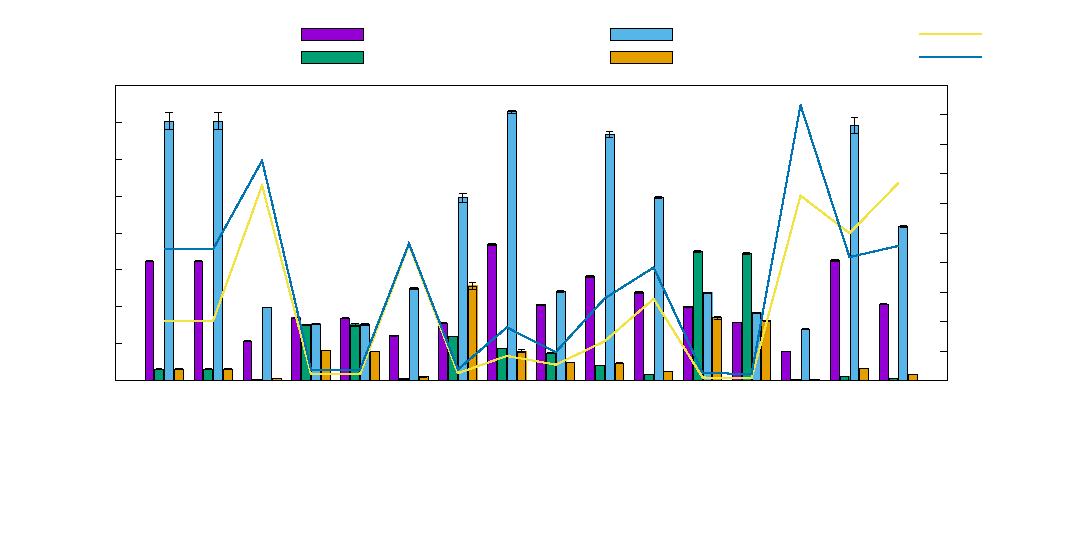
\includegraphics[width={504.00bp},height={252.00bp}]{all-hist-OnlineSetupTimesec}}%
    \gplfronttext
  \end{picture}%
\endgroup
}
% GNUPLOT: LaTeX picture with Postscript
\begingroup
  \makeatletter
  \providecommand\color[2][]{%
    \GenericError{(gnuplot) \space\space\space\@spaces}{%
      Package color not loaded in conjunction with
      terminal option `colourtext'%
    }{See the gnuplot documentation for explanation.%
    }{Either use 'blacktext' in gnuplot or load the package
      color.sty in LaTeX.}%
    \renewcommand\color[2][]{}%
  }%
  \providecommand\includegraphics[2][]{%
    \GenericError{(gnuplot) \space\space\space\@spaces}{%
      Package graphicx or graphics not loaded%
    }{See the gnuplot documentation for explanation.%
    }{The gnuplot epslatex terminal needs graphicx.sty or graphics.sty.}%
    \renewcommand\includegraphics[2][]{}%
  }%
  \providecommand\rotatebox[2]{#2}%
  \@ifundefined{ifGPcolor}{%
    \newif\ifGPcolor
    \GPcolortrue
  }{}%
  \@ifundefined{ifGPblacktext}{%
    \newif\ifGPblacktext
    \GPblacktextfalse
  }{}%
  % define a \g@addto@macro without @ in the name:
  \let\gplgaddtomacro\g@addto@macro
  % define empty templates for all commands taking text:
  \gdef\gplbacktext{}%
  \gdef\gplfronttext{}%
  \makeatother
  \ifGPblacktext
    % no textcolor at all
    \def\colorrgb#1{}%
    \def\colorgray#1{}%
  \else
    % gray or color?
    \ifGPcolor
      \def\colorrgb#1{\color[rgb]{#1}}%
      \def\colorgray#1{\color[gray]{#1}}%
      \expandafter\def\csname LTw\endcsname{\color{white}}%
      \expandafter\def\csname LTb\endcsname{\color{black}}%
      \expandafter\def\csname LTa\endcsname{\color{black}}%
      \expandafter\def\csname LT0\endcsname{\color[rgb]{1,0,0}}%
      \expandafter\def\csname LT1\endcsname{\color[rgb]{0,1,0}}%
      \expandafter\def\csname LT2\endcsname{\color[rgb]{0,0,1}}%
      \expandafter\def\csname LT3\endcsname{\color[rgb]{1,0,1}}%
      \expandafter\def\csname LT4\endcsname{\color[rgb]{0,1,1}}%
      \expandafter\def\csname LT5\endcsname{\color[rgb]{1,1,0}}%
      \expandafter\def\csname LT6\endcsname{\color[rgb]{0,0,0}}%
      \expandafter\def\csname LT7\endcsname{\color[rgb]{1,0.3,0}}%
      \expandafter\def\csname LT8\endcsname{\color[rgb]{0.5,0.5,0.5}}%
    \else
      % gray
      \def\colorrgb#1{\color{black}}%
      \def\colorgray#1{\color[gray]{#1}}%
      \expandafter\def\csname LTw\endcsname{\color{white}}%
      \expandafter\def\csname LTb\endcsname{\color{black}}%
      \expandafter\def\csname LTa\endcsname{\color{black}}%
      \expandafter\def\csname LT0\endcsname{\color{black}}%
      \expandafter\def\csname LT1\endcsname{\color{black}}%
      \expandafter\def\csname LT2\endcsname{\color{black}}%
      \expandafter\def\csname LT3\endcsname{\color{black}}%
      \expandafter\def\csname LT4\endcsname{\color{black}}%
      \expandafter\def\csname LT5\endcsname{\color{black}}%
      \expandafter\def\csname LT6\endcsname{\color{black}}%
      \expandafter\def\csname LT7\endcsname{\color{black}}%
      \expandafter\def\csname LT8\endcsname{\color{black}}%
    \fi
  \fi
    \setlength{\unitlength}{0.0500bp}%
    \ifx\gptboxheight\undefined%
      \newlength{\gptboxheight}%
      \newlength{\gptboxwidth}%
      \newsavebox{\gptboxtext}%
    \fi%
    \setlength{\fboxrule}{0.5pt}%
    \setlength{\fboxsep}{1pt}%
    \definecolor{tbcol}{rgb}{1,1,1}%
\begin{picture}(10080.00,5040.00)%
    \gplgaddtomacro\gplbacktext{%
      \csname LTb\endcsname%%
      \put(814,1540){\makebox(0,0)[r]{\strut{}$0$}}%
      \put(814,1895){\makebox(0,0)[r]{\strut{}$50$}}%
      \put(814,2250){\makebox(0,0)[r]{\strut{}$100$}}%
      \put(814,2605){\makebox(0,0)[r]{\strut{}$150$}}%
      \put(814,2960){\makebox(0,0)[r]{\strut{}$200$}}%
      \put(814,3314){\makebox(0,0)[r]{\strut{}$250$}}%
      \put(814,3669){\makebox(0,0)[r]{\strut{}$300$}}%
      \put(814,4024){\makebox(0,0)[r]{\strut{}$350$}}%
      \put(814,4379){\makebox(0,0)[r]{\strut{}$400$}}%
      \put(1416,1408){\rotatebox{-45}{\makebox(0,0)[l]{\strut{}Biometric Matching}}}%
      \put(1886,1408){\rotatebox{-45}{\makebox(0,0)[l]{\strut{}Biometric Matching (Fast)}}}%
      \put(2356,1408){\rotatebox{-45}{\makebox(0,0)[l]{\strut{}Convex Hull}}}%
      \put(2826,1408){\rotatebox{-45}{\makebox(0,0)[l]{\strut{}Count 102}}}%
      \put(3296,1408){\rotatebox{-45}{\makebox(0,0)[l]{\strut{}Count 10s}}}%
      \put(3766,1408){\rotatebox{-45}{\makebox(0,0)[l]{\strut{}Cryptonets (Max Pooling)}}}%
      \put(4236,1408){\rotatebox{-45}{\makebox(0,0)[l]{\strut{}Database Join}}}%
      \put(4706,1408){\rotatebox{-45}{\makebox(0,0)[l]{\strut{}Database Variance}}}%
      \put(5175,1408){\rotatebox{-45}{\makebox(0,0)[l]{\strut{}Histogram}}}%
      \put(5645,1408){\rotatebox{-45}{\makebox(0,0)[l]{\strut{}Inner Product}}}%
      \put(6115,1408){\rotatebox{-45}{\makebox(0,0)[l]{\strut{}k-means}}}%
      \put(6585,1408){\rotatebox{-45}{\makebox(0,0)[l]{\strut{}Longest 102}}}%
      \put(7055,1408){\rotatebox{-45}{\makebox(0,0)[l]{\strut{}Max. Dist. b/w Symbols}}}%
      \put(7525,1408){\rotatebox{-45}{\makebox(0,0)[l]{\strut{}Minimal Points}}}%
      \put(7995,1408){\rotatebox{-45}{\makebox(0,0)[l]{\strut{}MNIST ReLU}}}%
      \put(8465,1408){\rotatebox{-45}{\makebox(0,0)[l]{\strut{}Private Set Intersection}}}%
      \put(9067,1540){\makebox(0,0)[l]{\strut{}$0$}}%
      \put(9067,1946){\makebox(0,0)[l]{\strut{}$10$}}%
      \put(9067,2351){\makebox(0,0)[l]{\strut{}$20$}}%
      \put(9067,2757){\makebox(0,0)[l]{\strut{}$30$}}%
      \put(9067,3162){\makebox(0,0)[l]{\strut{}$40$}}%
      \put(9067,3568){\makebox(0,0)[l]{\strut{}$50$}}%
      \put(9067,3973){\makebox(0,0)[l]{\strut{}$60$}}%
      \put(9067,4379){\makebox(0,0)[l]{\strut{}$70$}}%
    }%
    \gplgaddtomacro\gplfronttext{%
      \csname LTb\endcsname%%
      \put(209,2959){\rotatebox{-270}{\makebox(0,0){\strut{}Online + Setup Time (sec)}}}%
      \put(9573,2959){\rotatebox{-270}{\makebox(0,0){\strut{}Improvement (number of times)}}}%
      \csname LTb\endcsname%%
      \put(2602,4867){\makebox(0,0)[r]{\strut{}GMW}}%
      \csname LTb\endcsname%%
      \put(2602,4647){\makebox(0,0)[r]{\strut{}GMW (Vectorized)}}%
      \csname LTb\endcsname%%
      \put(5569,4867){\makebox(0,0)[r]{\strut{}BMR}}%
      \csname LTb\endcsname%%
      \put(5569,4647){\makebox(0,0)[r]{\strut{}BMR (Vectorized)}}%
      \csname LTb\endcsname%%
      \put(8536,4867){\makebox(0,0)[r]{\strut{}GMW Improvement}}%
      \csname LTb\endcsname%%
      \put(8536,4647){\makebox(0,0)[r]{\strut{}BMR Improvement}}%
    }%
    \gplbacktext
    \put(0,0){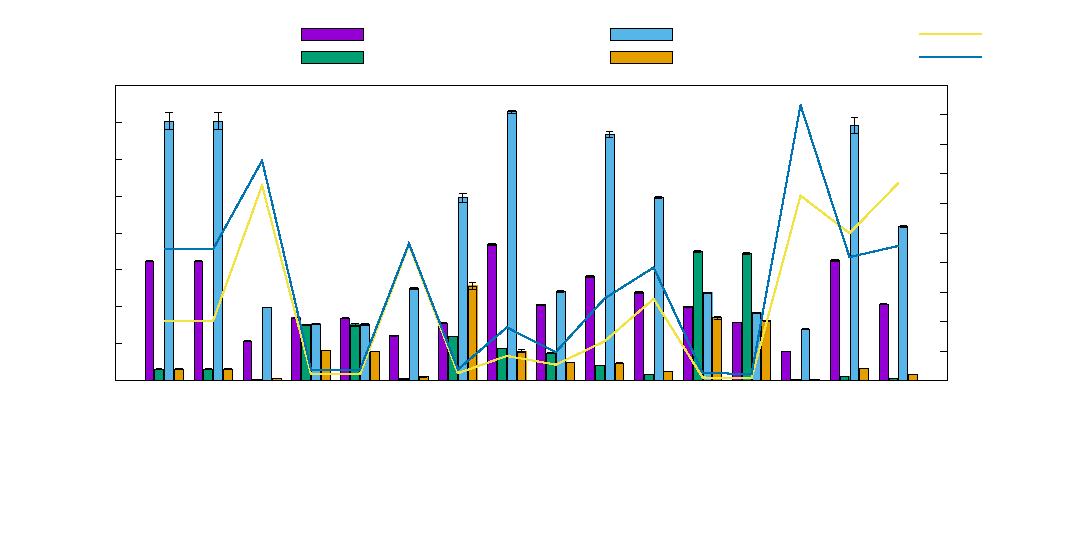
\includegraphics[width={504.00bp},height={252.00bp}]{all-hist-OnlineSetupTimesec}}%
    \gplfronttext
  \end{picture}%
\endgroup

\caption{Circuit Evaluation Time (Setup + Online) of Benchmarks}
\label{fig:graph_all_eval_time}
\end{figure*}

A detailed summary of the effects of vectorization on various benchmarks is presented in \cref{table:metrics}. We show circuit evaluation times in \cref{fig:graph_all_eval_time}. In terms of amenability to vectorization, we divide benchmarks into 3 categories: 1) {\it High:} these include convex hull, cryptonets max pooling, minimal points and private set intersection. These benchmarks are highly parallelizable and see 25x to 70x speedup in BMR, and 30x to 55x in GMW protocol. 2) {\it Medium:} these include biometric matching, DB Variance, histogram, inner product, k-means iteration and MNIST ReLU. These benchmarks have non-parallelizable phases e.g. the summing phase of inner product and biometric matching. Still, most computation is parallelizable and it results in speedup from 5x to 25x in BMR, and 2x to 25x in GMW protocol. 3) {\it Low:} these include the Database Join and the regular expression benchmarks (count 102, count 10, longest 102 and max distance between symbols). There is less parallelizable computation in these programs, thus the speedup is lower. We see a speedup from 1.1x to 2x in BMR. In GMW, DB Join, Count 102 and Count 10s see speedup from 1.1x to 1.3x. However, longest102 and max distance between symbols suffer a slowdown of 0.5x. There is opportunity for vectorization in these benchmarks according to our analytical model, particularly, a large EQ operation is vectorized, though a large portion of the loop cannot be vectorized. We observed that transformation to vectorized code increased multiplicative depth and, the negative effect of increased depth is more noticeable in a round-based protocol like GMW. The cause of the increase is not clear --- we conjecture that MOTION performs optimizations over the non-vectorized loop body that decreases depth; also, EQ is relatively inexpensive in Boolean GMW and BMR compared to ADD and MUL, which also de-emphasizes the benefit of vectorization. We propose a simple heuristic: if the transformation increases circuit depth beyond some threshold (e.g. more than 10\% of the original circuit), we reject the transformation. %Nevertheless, we show these graphs here for the sake of completeness and to highlight that vectorization is not always reduce run time. 
Note that in some settings it may still be desirable to vectorize e.g. in data constrained environments. As shown in \cref{fig:graph_comm_size}, vectorization results in reduced communication (fewer bits are transferred).

We present evaluation for communication size in \cref{fig:graph_comm_size}, circuit generation time in \cref{fig:graph_circ_gen_time}, number of gates in \cref{fig:graph_total_gates} and online time and setup time in \cref{fig:graph_online_time} and \cref{fig:graph_setup_time} respectively. %\ishaq{Ana: Let me know if I should add more substance.} \ana{It's good!}


\begin{figure}[htbp]
\centering
\resizebox{3.6in}{!}{% GNUPLOT: LaTeX picture with Postscript
\begingroup
  \makeatletter
  \providecommand\color[2][]{%
    \GenericError{(gnuplot) \space\space\space\@spaces}{%
      Package color not loaded in conjunction with
      terminal option `colourtext'%
    }{See the gnuplot documentation for explanation.%
    }{Either use 'blacktext' in gnuplot or load the package
      color.sty in LaTeX.}%
    \renewcommand\color[2][]{}%
  }%
  \providecommand\includegraphics[2][]{%
    \GenericError{(gnuplot) \space\space\space\@spaces}{%
      Package graphicx or graphics not loaded%
    }{See the gnuplot documentation for explanation.%
    }{The gnuplot epslatex terminal needs graphicx.sty or graphics.sty.}%
    \renewcommand\includegraphics[2][]{}%
  }%
  \providecommand\rotatebox[2]{#2}%
  \@ifundefined{ifGPcolor}{%
    \newif\ifGPcolor
    \GPcolortrue
  }{}%
  \@ifundefined{ifGPblacktext}{%
    \newif\ifGPblacktext
    \GPblacktextfalse
  }{}%
  % define a \g@addto@macro without @ in the name:
  \let\gplgaddtomacro\g@addto@macro
  % define empty templates for all commands taking text:
  \gdef\gplbacktext{}%
  \gdef\gplfronttext{}%
  \makeatother
  \ifGPblacktext
    % no textcolor at all
    \def\colorrgb#1{}%
    \def\colorgray#1{}%
  \else
    % gray or color?
    \ifGPcolor
      \def\colorrgb#1{\color[rgb]{#1}}%
      \def\colorgray#1{\color[gray]{#1}}%
      \expandafter\def\csname LTw\endcsname{\color{white}}%
      \expandafter\def\csname LTb\endcsname{\color{black}}%
      \expandafter\def\csname LTa\endcsname{\color{black}}%
      \expandafter\def\csname LT0\endcsname{\color[rgb]{1,0,0}}%
      \expandafter\def\csname LT1\endcsname{\color[rgb]{0,1,0}}%
      \expandafter\def\csname LT2\endcsname{\color[rgb]{0,0,1}}%
      \expandafter\def\csname LT3\endcsname{\color[rgb]{1,0,1}}%
      \expandafter\def\csname LT4\endcsname{\color[rgb]{0,1,1}}%
      \expandafter\def\csname LT5\endcsname{\color[rgb]{1,1,0}}%
      \expandafter\def\csname LT6\endcsname{\color[rgb]{0,0,0}}%
      \expandafter\def\csname LT7\endcsname{\color[rgb]{1,0.3,0}}%
      \expandafter\def\csname LT8\endcsname{\color[rgb]{0.5,0.5,0.5}}%
    \else
      % gray
      \def\colorrgb#1{\color{black}}%
      \def\colorgray#1{\color[gray]{#1}}%
      \expandafter\def\csname LTw\endcsname{\color{white}}%
      \expandafter\def\csname LTb\endcsname{\color{black}}%
      \expandafter\def\csname LTa\endcsname{\color{black}}%
      \expandafter\def\csname LT0\endcsname{\color{black}}%
      \expandafter\def\csname LT1\endcsname{\color{black}}%
      \expandafter\def\csname LT2\endcsname{\color{black}}%
      \expandafter\def\csname LT3\endcsname{\color{black}}%
      \expandafter\def\csname LT4\endcsname{\color{black}}%
      \expandafter\def\csname LT5\endcsname{\color{black}}%
      \expandafter\def\csname LT6\endcsname{\color{black}}%
      \expandafter\def\csname LT7\endcsname{\color{black}}%
      \expandafter\def\csname LT8\endcsname{\color{black}}%
    \fi
  \fi
    \setlength{\unitlength}{0.0500bp}%
    \ifx\gptboxheight\undefined%
      \newlength{\gptboxheight}%
      \newlength{\gptboxwidth}%
      \newsavebox{\gptboxtext}%
    \fi%
    \setlength{\fboxrule}{0.5pt}%
    \setlength{\fboxsep}{1pt}%
    \definecolor{tbcol}{rgb}{1,1,1}%
\begin{picture}(5760.00,4320.00)%
    \gplgaddtomacro\gplbacktext{%
      \csname LTb\endcsname%%
      \put(814,440){\makebox(0,0)[r]{\strut{}$0$}}%
      \put(814,806){\makebox(0,0)[r]{\strut{}$50$}}%
      \put(814,1172){\makebox(0,0)[r]{\strut{}$100$}}%
      \put(814,1538){\makebox(0,0)[r]{\strut{}$150$}}%
      \put(814,1904){\makebox(0,0)[r]{\strut{}$200$}}%
      \put(814,2270){\makebox(0,0)[r]{\strut{}$250$}}%
      \put(814,2635){\makebox(0,0)[r]{\strut{}$300$}}%
      \put(814,3001){\makebox(0,0)[r]{\strut{}$350$}}%
      \put(814,3367){\makebox(0,0)[r]{\strut{}$400$}}%
      \put(814,3733){\makebox(0,0)[r]{\strut{}$450$}}%
      \put(814,4099){\makebox(0,0)[r]{\strut{}$500$}}%
      \put(1252,308){\rotatebox{-45}{\makebox(0,0)[l]{\strut{}N: 4}}}%
      \put(1558,308){\rotatebox{-45}{\makebox(0,0)[l]{\strut{}N: 8}}}%
      \put(1863,308){\rotatebox{-45}{\makebox(0,0)[l]{\strut{}N: 16}}}%
      \put(2169,308){\rotatebox{-45}{\makebox(0,0)[l]{\strut{}N: 32}}}%
      \put(2475,308){\rotatebox{-45}{\makebox(0,0)[l]{\strut{}N: 64}}}%
      \put(2781,308){\rotatebox{-45}{\makebox(0,0)[l]{\strut{}N: 128}}}%
      \put(3086,308){\rotatebox{-45}{\makebox(0,0)[l]{\strut{}N: 256}}}%
      \put(3392,308){\rotatebox{-45}{\makebox(0,0)[l]{\strut{}N: 512}}}%
      \put(3698,308){\rotatebox{-45}{\makebox(0,0)[l]{\strut{}N: 1024}}}%
      \put(4004,308){\rotatebox{-45}{\makebox(0,0)[l]{\strut{}N: 2048}}}%
      \put(4309,308){\rotatebox{-45}{\makebox(0,0)[l]{\strut{}N: 4096}}}%
      \put(4747,440){\makebox(0,0)[l]{\strut{}$0$}}%
      \put(4747,1172){\makebox(0,0)[l]{\strut{}$5$}}%
      \put(4747,1904){\makebox(0,0)[l]{\strut{}$10$}}%
      \put(4747,2635){\makebox(0,0)[l]{\strut{}$15$}}%
      \put(4747,3367){\makebox(0,0)[l]{\strut{}$20$}}%
      \put(4747,4099){\makebox(0,0)[l]{\strut{}$25$}}%
    }%
    \gplgaddtomacro\gplfronttext{%
      \csname LTb\endcsname%%
      \put(209,2269){\rotatebox{-270}{\makebox(0,0){\strut{}Online + Setup Time (sec)}}}%
      \put(5253,2269){\rotatebox{-270}{\makebox(0,0){\strut{}Improvement (number of times)}}}%
      \csname LTb\endcsname%%
      \put(3190,3926){\makebox(0,0)[r]{\strut{}GMW}}%
      \csname LTb\endcsname%%
      \put(3190,3706){\makebox(0,0)[r]{\strut{}GMW (Vectorized)}}%
      \csname LTb\endcsname%%
      \put(3190,3486){\makebox(0,0)[r]{\strut{}BMR}}%
      \csname LTb\endcsname%%
      \put(3190,3266){\makebox(0,0)[r]{\strut{}BMR (Vectorized)}}%
      \csname LTb\endcsname%%
      \put(3190,3046){\makebox(0,0)[r]{\strut{}GMW Improvement}}%
      \csname LTb\endcsname%%
      \put(3190,2826){\makebox(0,0)[r]{\strut{}BMR Improvement}}%
    }%
    \gplbacktext
    \put(0,0){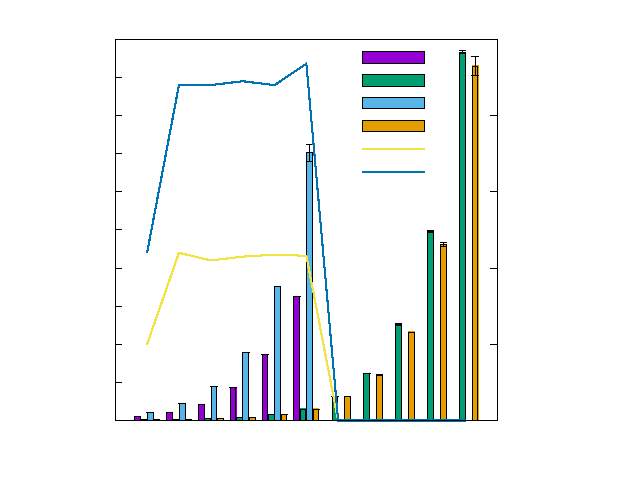
\includegraphics[width={288.00bp},height={216.00bp}]{biometric-hist-OnlineSetupTimesec}}%
    \gplfronttext
  \end{picture}%
\endgroup
}
\caption{Biometric Matching Circuit Evaluation Time, x-axis lists database size}
\label{fig:graph_biometric_eval_time}
\end{figure}

\begin{figure}[htbp]
\centering
\resizebox{3.6in}{!}{% GNUPLOT: LaTeX picture with Postscript
\begingroup
  \makeatletter
  \providecommand\color[2][]{%
    \GenericError{(gnuplot) \space\space\space\@spaces}{%
      Package color not loaded in conjunction with
      terminal option `colourtext'%
    }{See the gnuplot documentation for explanation.%
    }{Either use 'blacktext' in gnuplot or load the package
      color.sty in LaTeX.}%
    \renewcommand\color[2][]{}%
  }%
  \providecommand\includegraphics[2][]{%
    \GenericError{(gnuplot) \space\space\space\@spaces}{%
      Package graphicx or graphics not loaded%
    }{See the gnuplot documentation for explanation.%
    }{The gnuplot epslatex terminal needs graphicx.sty or graphics.sty.}%
    \renewcommand\includegraphics[2][]{}%
  }%
  \providecommand\rotatebox[2]{#2}%
  \@ifundefined{ifGPcolor}{%
    \newif\ifGPcolor
    \GPcolortrue
  }{}%
  \@ifundefined{ifGPblacktext}{%
    \newif\ifGPblacktext
    \GPblacktextfalse
  }{}%
  % define a \g@addto@macro without @ in the name:
  \let\gplgaddtomacro\g@addto@macro
  % define empty templates for all commands taking text:
  \gdef\gplbacktext{}%
  \gdef\gplfronttext{}%
  \makeatother
  \ifGPblacktext
    % no textcolor at all
    \def\colorrgb#1{}%
    \def\colorgray#1{}%
  \else
    % gray or color?
    \ifGPcolor
      \def\colorrgb#1{\color[rgb]{#1}}%
      \def\colorgray#1{\color[gray]{#1}}%
      \expandafter\def\csname LTw\endcsname{\color{white}}%
      \expandafter\def\csname LTb\endcsname{\color{black}}%
      \expandafter\def\csname LTa\endcsname{\color{black}}%
      \expandafter\def\csname LT0\endcsname{\color[rgb]{1,0,0}}%
      \expandafter\def\csname LT1\endcsname{\color[rgb]{0,1,0}}%
      \expandafter\def\csname LT2\endcsname{\color[rgb]{0,0,1}}%
      \expandafter\def\csname LT3\endcsname{\color[rgb]{1,0,1}}%
      \expandafter\def\csname LT4\endcsname{\color[rgb]{0,1,1}}%
      \expandafter\def\csname LT5\endcsname{\color[rgb]{1,1,0}}%
      \expandafter\def\csname LT6\endcsname{\color[rgb]{0,0,0}}%
      \expandafter\def\csname LT7\endcsname{\color[rgb]{1,0.3,0}}%
      \expandafter\def\csname LT8\endcsname{\color[rgb]{0.5,0.5,0.5}}%
    \else
      % gray
      \def\colorrgb#1{\color{black}}%
      \def\colorgray#1{\color[gray]{#1}}%
      \expandafter\def\csname LTw\endcsname{\color{white}}%
      \expandafter\def\csname LTb\endcsname{\color{black}}%
      \expandafter\def\csname LTa\endcsname{\color{black}}%
      \expandafter\def\csname LT0\endcsname{\color{black}}%
      \expandafter\def\csname LT1\endcsname{\color{black}}%
      \expandafter\def\csname LT2\endcsname{\color{black}}%
      \expandafter\def\csname LT3\endcsname{\color{black}}%
      \expandafter\def\csname LT4\endcsname{\color{black}}%
      \expandafter\def\csname LT5\endcsname{\color{black}}%
      \expandafter\def\csname LT6\endcsname{\color{black}}%
      \expandafter\def\csname LT7\endcsname{\color{black}}%
      \expandafter\def\csname LT8\endcsname{\color{black}}%
    \fi
  \fi
    \setlength{\unitlength}{0.0500bp}%
    \ifx\gptboxheight\undefined%
      \newlength{\gptboxheight}%
      \newlength{\gptboxwidth}%
      \newsavebox{\gptboxtext}%
    \fi%
    \setlength{\fboxrule}{0.5pt}%
    \setlength{\fboxsep}{1pt}%
    \definecolor{tbcol}{rgb}{1,1,1}%
\begin{picture}(5760.00,4320.00)%
    \gplgaddtomacro\gplbacktext{%
      \csname LTb\endcsname%%
      \put(946,440){\makebox(0,0)[r]{\strut{}$0$}}%
      \put(946,847){\makebox(0,0)[r]{\strut{}$500$}}%
      \put(946,1253){\makebox(0,0)[r]{\strut{}$1000$}}%
      \put(946,1660){\makebox(0,0)[r]{\strut{}$1500$}}%
      \put(946,2066){\makebox(0,0)[r]{\strut{}$2000$}}%
      \put(946,2473){\makebox(0,0)[r]{\strut{}$2500$}}%
      \put(946,2879){\makebox(0,0)[r]{\strut{}$3000$}}%
      \put(946,3286){\makebox(0,0)[r]{\strut{}$3500$}}%
      \put(946,3692){\makebox(0,0)[r]{\strut{}$4000$}}%
      \put(946,4099){\makebox(0,0)[r]{\strut{}$4500$}}%
      \put(1373,308){\rotatebox{-45}{\makebox(0,0)[l]{\strut{}N: 4}}}%
      \put(1668,308){\rotatebox{-45}{\makebox(0,0)[l]{\strut{}N: 8}}}%
      \put(1962,308){\rotatebox{-45}{\makebox(0,0)[l]{\strut{}N: 16}}}%
      \put(2257,308){\rotatebox{-45}{\makebox(0,0)[l]{\strut{}N: 32}}}%
      \put(2552,308){\rotatebox{-45}{\makebox(0,0)[l]{\strut{}N: 64}}}%
      \put(2847,308){\rotatebox{-45}{\makebox(0,0)[l]{\strut{}N: 128}}}%
      \put(3141,308){\rotatebox{-45}{\makebox(0,0)[l]{\strut{}N: 256}}}%
      \put(3436,308){\rotatebox{-45}{\makebox(0,0)[l]{\strut{}N: 512}}}%
      \put(3731,308){\rotatebox{-45}{\makebox(0,0)[l]{\strut{}N: 1024}}}%
      \put(4026,308){\rotatebox{-45}{\makebox(0,0)[l]{\strut{}N: 2048}}}%
      \put(4320,308){\rotatebox{-45}{\makebox(0,0)[l]{\strut{}N: 4096}}}%
      \put(4747,440){\makebox(0,0)[l]{\strut{}$0$}}%
      \put(4747,1050){\makebox(0,0)[l]{\strut{}$2$}}%
      \put(4747,1660){\makebox(0,0)[l]{\strut{}$4$}}%
      \put(4747,2270){\makebox(0,0)[l]{\strut{}$6$}}%
      \put(4747,2879){\makebox(0,0)[l]{\strut{}$8$}}%
      \put(4747,3489){\makebox(0,0)[l]{\strut{}$10$}}%
      \put(4747,4099){\makebox(0,0)[l]{\strut{}$12$}}%
    }%
    \gplgaddtomacro\gplfronttext{%
      \csname LTb\endcsname%%
      \put(209,2269){\rotatebox{-270}{\makebox(0,0){\strut{}Communication (MiB)}}}%
      \put(5253,2269){\rotatebox{-270}{\makebox(0,0){\strut{}Improvement (number of times)}}}%
      \csname LTb\endcsname%%
      \put(3322,3926){\makebox(0,0)[r]{\strut{}GMW}}%
      \csname LTb\endcsname%%
      \put(3322,3706){\makebox(0,0)[r]{\strut{}GMW (Vectorized)}}%
      \csname LTb\endcsname%%
      \put(3322,3486){\makebox(0,0)[r]{\strut{}BMR}}%
      \csname LTb\endcsname%%
      \put(3322,3266){\makebox(0,0)[r]{\strut{}BMR (Vectorized)}}%
      \csname LTb\endcsname%%
      \put(3322,3046){\makebox(0,0)[r]{\strut{}GMW Improvement}}%
      \csname LTb\endcsname%%
      \put(3322,2826){\makebox(0,0)[r]{\strut{}BMR Improvement}}%
    }%
    \gplbacktext
    \put(0,0){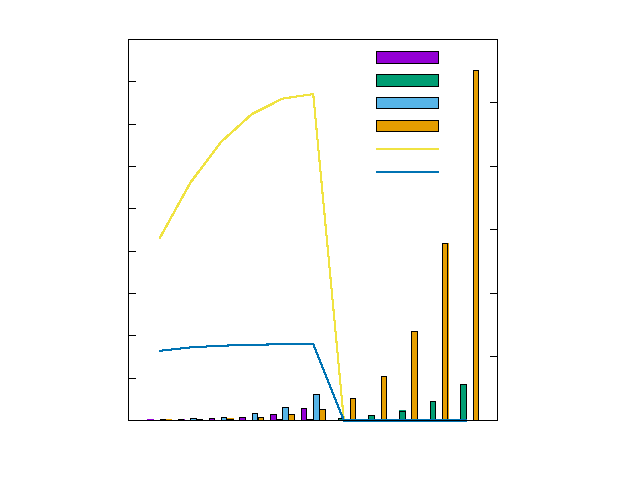
\includegraphics[width={288.00bp},height={216.00bp}]{biometric-hist-CommunicationMiB}}%
    \gplfronttext
  \end{picture}%
\endgroup
}
\caption{Biometric Matching Communication Size, x-axis lists database size}
\label{fig:graph_biometic_comm_size}
\end{figure}

\begin{figure}[htbp]
\centering
\resizebox{3.6in}{!}{% GNUPLOT: LaTeX picture with Postscript
\begingroup
  \makeatletter
  \providecommand\color[2][]{%
    \GenericError{(gnuplot) \space\space\space\@spaces}{%
      Package color not loaded in conjunction with
      terminal option `colourtext'%
    }{See the gnuplot documentation for explanation.%
    }{Either use 'blacktext' in gnuplot or load the package
      color.sty in LaTeX.}%
    \renewcommand\color[2][]{}%
  }%
  \providecommand\includegraphics[2][]{%
    \GenericError{(gnuplot) \space\space\space\@spaces}{%
      Package graphicx or graphics not loaded%
    }{See the gnuplot documentation for explanation.%
    }{The gnuplot epslatex terminal needs graphicx.sty or graphics.sty.}%
    \renewcommand\includegraphics[2][]{}%
  }%
  \providecommand\rotatebox[2]{#2}%
  \@ifundefined{ifGPcolor}{%
    \newif\ifGPcolor
    \GPcolortrue
  }{}%
  \@ifundefined{ifGPblacktext}{%
    \newif\ifGPblacktext
    \GPblacktextfalse
  }{}%
  % define a \g@addto@macro without @ in the name:
  \let\gplgaddtomacro\g@addto@macro
  % define empty templates for all commands taking text:
  \gdef\gplbacktext{}%
  \gdef\gplfronttext{}%
  \makeatother
  \ifGPblacktext
    % no textcolor at all
    \def\colorrgb#1{}%
    \def\colorgray#1{}%
  \else
    % gray or color?
    \ifGPcolor
      \def\colorrgb#1{\color[rgb]{#1}}%
      \def\colorgray#1{\color[gray]{#1}}%
      \expandafter\def\csname LTw\endcsname{\color{white}}%
      \expandafter\def\csname LTb\endcsname{\color{black}}%
      \expandafter\def\csname LTa\endcsname{\color{black}}%
      \expandafter\def\csname LT0\endcsname{\color[rgb]{1,0,0}}%
      \expandafter\def\csname LT1\endcsname{\color[rgb]{0,1,0}}%
      \expandafter\def\csname LT2\endcsname{\color[rgb]{0,0,1}}%
      \expandafter\def\csname LT3\endcsname{\color[rgb]{1,0,1}}%
      \expandafter\def\csname LT4\endcsname{\color[rgb]{0,1,1}}%
      \expandafter\def\csname LT5\endcsname{\color[rgb]{1,1,0}}%
      \expandafter\def\csname LT6\endcsname{\color[rgb]{0,0,0}}%
      \expandafter\def\csname LT7\endcsname{\color[rgb]{1,0.3,0}}%
      \expandafter\def\csname LT8\endcsname{\color[rgb]{0.5,0.5,0.5}}%
    \else
      % gray
      \def\colorrgb#1{\color{black}}%
      \def\colorgray#1{\color[gray]{#1}}%
      \expandafter\def\csname LTw\endcsname{\color{white}}%
      \expandafter\def\csname LTb\endcsname{\color{black}}%
      \expandafter\def\csname LTa\endcsname{\color{black}}%
      \expandafter\def\csname LT0\endcsname{\color{black}}%
      \expandafter\def\csname LT1\endcsname{\color{black}}%
      \expandafter\def\csname LT2\endcsname{\color{black}}%
      \expandafter\def\csname LT3\endcsname{\color{black}}%
      \expandafter\def\csname LT4\endcsname{\color{black}}%
      \expandafter\def\csname LT5\endcsname{\color{black}}%
      \expandafter\def\csname LT6\endcsname{\color{black}}%
      \expandafter\def\csname LT7\endcsname{\color{black}}%
      \expandafter\def\csname LT8\endcsname{\color{black}}%
    \fi
  \fi
    \setlength{\unitlength}{0.0500bp}%
    \ifx\gptboxheight\undefined%
      \newlength{\gptboxheight}%
      \newlength{\gptboxwidth}%
      \newsavebox{\gptboxtext}%
    \fi%
    \setlength{\fboxrule}{0.5pt}%
    \setlength{\fboxsep}{1pt}%
    \definecolor{tbcol}{rgb}{1,1,1}%
\begin{picture}(5760.00,4320.00)%
    \gplgaddtomacro\gplbacktext{%
      \csname LTb\endcsname%%
      \put(814,440){\makebox(0,0)[r]{\strut{}$0$}}%
      \put(814,963){\makebox(0,0)[r]{\strut{}$20$}}%
      \put(814,1485){\makebox(0,0)[r]{\strut{}$40$}}%
      \put(814,2008){\makebox(0,0)[r]{\strut{}$60$}}%
      \put(814,2531){\makebox(0,0)[r]{\strut{}$80$}}%
      \put(814,3054){\makebox(0,0)[r]{\strut{}$100$}}%
      \put(814,3576){\makebox(0,0)[r]{\strut{}$120$}}%
      \put(814,4099){\makebox(0,0)[r]{\strut{}$140$}}%
      \put(1252,308){\rotatebox{-45}{\makebox(0,0)[l]{\strut{}N: 4}}}%
      \put(1558,308){\rotatebox{-45}{\makebox(0,0)[l]{\strut{}N: 8}}}%
      \put(1863,308){\rotatebox{-45}{\makebox(0,0)[l]{\strut{}N: 16}}}%
      \put(2169,308){\rotatebox{-45}{\makebox(0,0)[l]{\strut{}N: 32}}}%
      \put(2475,308){\rotatebox{-45}{\makebox(0,0)[l]{\strut{}N: 64}}}%
      \put(2781,308){\rotatebox{-45}{\makebox(0,0)[l]{\strut{}N: 128}}}%
      \put(3086,308){\rotatebox{-45}{\makebox(0,0)[l]{\strut{}N: 256}}}%
      \put(3392,308){\rotatebox{-45}{\makebox(0,0)[l]{\strut{}N: 512}}}%
      \put(3698,308){\rotatebox{-45}{\makebox(0,0)[l]{\strut{}N: 1024}}}%
      \put(4004,308){\rotatebox{-45}{\makebox(0,0)[l]{\strut{}N: 2048}}}%
      \put(4309,308){\rotatebox{-45}{\makebox(0,0)[l]{\strut{}N: 4096}}}%
      \put(4747,440){\makebox(0,0)[l]{\strut{}$0$}}%
      \put(4747,963){\makebox(0,0)[l]{\strut{}$10$}}%
      \put(4747,1485){\makebox(0,0)[l]{\strut{}$20$}}%
      \put(4747,2008){\makebox(0,0)[l]{\strut{}$30$}}%
      \put(4747,2531){\makebox(0,0)[l]{\strut{}$40$}}%
      \put(4747,3054){\makebox(0,0)[l]{\strut{}$50$}}%
      \put(4747,3576){\makebox(0,0)[l]{\strut{}$60$}}%
      \put(4747,4099){\makebox(0,0)[l]{\strut{}$70$}}%
    }%
    \gplgaddtomacro\gplfronttext{%
      \csname LTb\endcsname%%
      \put(209,2269){\rotatebox{-270}{\makebox(0,0){\strut{}Circuit Generation Time (sec)}}}%
      \put(5253,2269){\rotatebox{-270}{\makebox(0,0){\strut{}Improvement (number of times)}}}%
      \csname LTb\endcsname%%
      \put(3190,3926){\makebox(0,0)[r]{\strut{}GMW}}%
      \csname LTb\endcsname%%
      \put(3190,3706){\makebox(0,0)[r]{\strut{}GMW (Vectorized)}}%
      \csname LTb\endcsname%%
      \put(3190,3486){\makebox(0,0)[r]{\strut{}BMR}}%
      \csname LTb\endcsname%%
      \put(3190,3266){\makebox(0,0)[r]{\strut{}BMR (Vectorized)}}%
      \csname LTb\endcsname%%
      \put(3190,3046){\makebox(0,0)[r]{\strut{}GMW Improvement}}%
      \csname LTb\endcsname%%
      \put(3190,2826){\makebox(0,0)[r]{\strut{}BMR Improvement}}%
    }%
    \gplbacktext
    \put(0,0){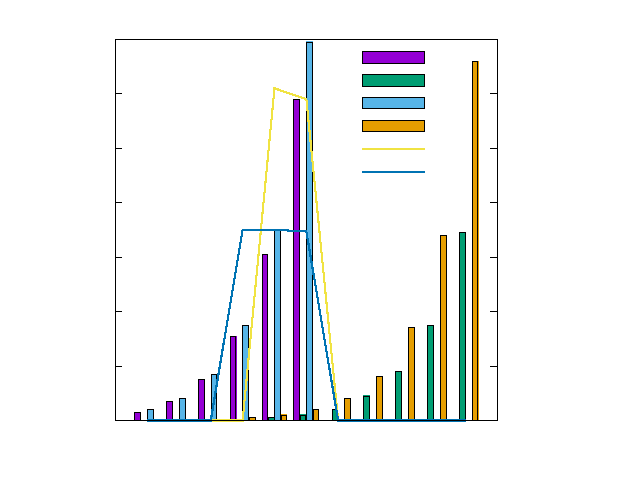
\includegraphics[width={288.00bp},height={216.00bp}]{biometric-hist-CircuitGenerationTimesec}}%
    \gplfronttext
  \end{picture}%
\endgroup
}
\caption{Biometric Matching Circuit Generation Time, x-axis lists database size}
\label{fig:graph_biometic_circ_gen_time}
\end{figure}

We look closely at the Biometric Matching benchmark: circuit evaluation in~\cref{fig:graph_biometric_eval_time}, communication size in \cref{fig:graph_biometic_comm_size} and circuit generation time in~\cref{fig:graph_biometic_circ_gen_time}. For input size beyond {\tt N=128} the memory usage exceeds available memory and prevents circuit generation. Consequently, non-vectorized bars are missing beyond this threshold. Notice that vectorization improves all metrics. %A database of size {\tt N=128} is smaller than any real world use case, therefore lets use it as baseline for improvement. 
Comparing performance improvement between BMR and GMW, we see more speedup for BMR (23x vs 10x), GMW gets more communication size reduction (10x vs 2.5x) and circuit generation sees a speedup of 35x and 45x for BMR and GMW respectively. 



\begin{figure}[htbp]
\centering
\resizebox{3.6in}{!}{% GNUPLOT: LaTeX picture with Postscript
\begingroup
  \makeatletter
  \providecommand\color[2][]{%
    \GenericError{(gnuplot) \space\space\space\@spaces}{%
      Package color not loaded in conjunction with
      terminal option `colourtext'%
    }{See the gnuplot documentation for explanation.%
    }{Either use 'blacktext' in gnuplot or load the package
      color.sty in LaTeX.}%
    \renewcommand\color[2][]{}%
  }%
  \providecommand\includegraphics[2][]{%
    \GenericError{(gnuplot) \space\space\space\@spaces}{%
      Package graphicx or graphics not loaded%
    }{See the gnuplot documentation for explanation.%
    }{The gnuplot epslatex terminal needs graphicx.sty or graphics.sty.}%
    \renewcommand\includegraphics[2][]{}%
  }%
  \providecommand\rotatebox[2]{#2}%
  \@ifundefined{ifGPcolor}{%
    \newif\ifGPcolor
    \GPcolortrue
  }{}%
  \@ifundefined{ifGPblacktext}{%
    \newif\ifGPblacktext
    \GPblacktextfalse
  }{}%
  % define a \g@addto@macro without @ in the name:
  \let\gplgaddtomacro\g@addto@macro
  % define empty templates for all commands taking text:
  \gdef\gplbacktext{}%
  \gdef\gplfronttext{}%
  \makeatother
  \ifGPblacktext
    % no textcolor at all
    \def\colorrgb#1{}%
    \def\colorgray#1{}%
  \else
    % gray or color?
    \ifGPcolor
      \def\colorrgb#1{\color[rgb]{#1}}%
      \def\colorgray#1{\color[gray]{#1}}%
      \expandafter\def\csname LTw\endcsname{\color{white}}%
      \expandafter\def\csname LTb\endcsname{\color{black}}%
      \expandafter\def\csname LTa\endcsname{\color{black}}%
      \expandafter\def\csname LT0\endcsname{\color[rgb]{1,0,0}}%
      \expandafter\def\csname LT1\endcsname{\color[rgb]{0,1,0}}%
      \expandafter\def\csname LT2\endcsname{\color[rgb]{0,0,1}}%
      \expandafter\def\csname LT3\endcsname{\color[rgb]{1,0,1}}%
      \expandafter\def\csname LT4\endcsname{\color[rgb]{0,1,1}}%
      \expandafter\def\csname LT5\endcsname{\color[rgb]{1,1,0}}%
      \expandafter\def\csname LT6\endcsname{\color[rgb]{0,0,0}}%
      \expandafter\def\csname LT7\endcsname{\color[rgb]{1,0.3,0}}%
      \expandafter\def\csname LT8\endcsname{\color[rgb]{0.5,0.5,0.5}}%
    \else
      % gray
      \def\colorrgb#1{\color{black}}%
      \def\colorgray#1{\color[gray]{#1}}%
      \expandafter\def\csname LTw\endcsname{\color{white}}%
      \expandafter\def\csname LTb\endcsname{\color{black}}%
      \expandafter\def\csname LTa\endcsname{\color{black}}%
      \expandafter\def\csname LT0\endcsname{\color{black}}%
      \expandafter\def\csname LT1\endcsname{\color{black}}%
      \expandafter\def\csname LT2\endcsname{\color{black}}%
      \expandafter\def\csname LT3\endcsname{\color{black}}%
      \expandafter\def\csname LT4\endcsname{\color{black}}%
      \expandafter\def\csname LT5\endcsname{\color{black}}%
      \expandafter\def\csname LT6\endcsname{\color{black}}%
      \expandafter\def\csname LT7\endcsname{\color{black}}%
      \expandafter\def\csname LT8\endcsname{\color{black}}%
    \fi
  \fi
    \setlength{\unitlength}{0.0500bp}%
    \ifx\gptboxheight\undefined%
      \newlength{\gptboxheight}%
      \newlength{\gptboxwidth}%
      \newsavebox{\gptboxtext}%
    \fi%
    \setlength{\fboxrule}{0.5pt}%
    \setlength{\fboxsep}{1pt}%
    \definecolor{tbcol}{rgb}{1,1,1}%
\begin{picture}(5760.00,4320.00)%
    \gplgaddtomacro\gplbacktext{%
      \csname LTb\endcsname%%
      \put(946,1100){\makebox(0,0)[r]{\strut{}$0$}}%
      \csname LTb\endcsname%%
      \put(946,1528){\makebox(0,0)[r]{\strut{}$500$}}%
      \csname LTb\endcsname%%
      \put(946,1957){\makebox(0,0)[r]{\strut{}$1000$}}%
      \csname LTb\endcsname%%
      \put(946,2385){\makebox(0,0)[r]{\strut{}$1500$}}%
      \csname LTb\endcsname%%
      \put(946,2814){\makebox(0,0)[r]{\strut{}$2000$}}%
      \csname LTb\endcsname%%
      \put(946,3242){\makebox(0,0)[r]{\strut{}$2500$}}%
      \csname LTb\endcsname%%
      \put(946,3671){\makebox(0,0)[r]{\strut{}$3000$}}%
      \csname LTb\endcsname%%
      \put(946,4099){\makebox(0,0)[r]{\strut{}$3500$}}%
      \csname LTb\endcsname%%
      \put(1902,968){\rotatebox{-25}{\makebox(0,0)[l]{\strut{}Biometric Matching}}}%
      \csname LTb\endcsname%%
      \put(2725,968){\rotatebox{-25}{\makebox(0,0)[l]{\strut{}Biometric Matching (Fast)}}}%
      \csname LTb\endcsname%%
      \put(3549,968){\rotatebox{-25}{\makebox(0,0)[l]{\strut{}Inner Product}}}%
      \csname LTb\endcsname%%
      \put(4372,968){\rotatebox{-25}{\makebox(0,0)[l]{\strut{}Longest 102}}}%
    }%
    \gplgaddtomacro\gplfronttext{%
      \csname LTb\endcsname%%
      \put(209,2599){\rotatebox{-270}{\makebox(0,0){\strut{}Online + Setup Time (sec)}}}%
      \csname LTb\endcsname%%
      \put(4209,3926){\makebox(0,0)[r]{\strut{}GMW LAN}}%
      \csname LTb\endcsname%%
      \put(4209,3706){\makebox(0,0)[r]{\strut{}GMW WAN}}%
      \csname LTb\endcsname%%
      \put(4209,3486){\makebox(0,0)[r]{\strut{}BMR LAN}}%
      \csname LTb\endcsname%%
      \put(4209,3266){\makebox(0,0)[r]{\strut{}BMR WAN}}%
    }%
    \gplbacktext
    \put(0,0){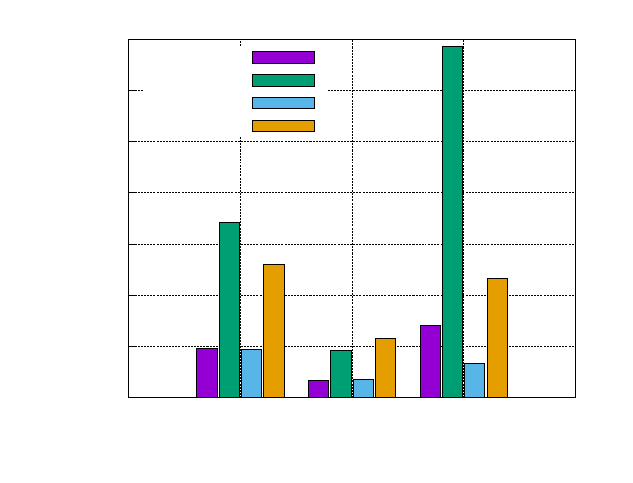
\includegraphics[width={288.00bp},height={216.00bp}]{comparison-hist-OnlineSetupTimesec}}%
    \gplfronttext
  \end{picture}%
\endgroup
}
\caption{LAN vs. WAN: Circuit Evaluation Time Comparison}
\label{fig:graph_comparison_eval_time}
\end{figure}

Since our vectorization framework is network agnostic, it produces the same circuit for both LAN and WAN. This means that the number of gates and communication size remain the same. Moreover, time for circuit generation, which is a local operation, also remains unchanged. Setup and Online times, however, increase due to lower bandwidth and higher latency of the WAN. Indeed, this is what we observe in \cref{fig:graph_comparison_eval_time}.

\begin{figure*}[htbp]
\centering
% GNUPLOT: LaTeX picture with Postscript
\begingroup
  \makeatletter
  \providecommand\color[2][]{%
    \GenericError{(gnuplot) \space\space\space\@spaces}{%
      Package color not loaded in conjunction with
      terminal option `colourtext'%
    }{See the gnuplot documentation for explanation.%
    }{Either use 'blacktext' in gnuplot or load the package
      color.sty in LaTeX.}%
    \renewcommand\color[2][]{}%
  }%
  \providecommand\includegraphics[2][]{%
    \GenericError{(gnuplot) \space\space\space\@spaces}{%
      Package graphicx or graphics not loaded%
    }{See the gnuplot documentation for explanation.%
    }{The gnuplot epslatex terminal needs graphicx.sty or graphics.sty.}%
    \renewcommand\includegraphics[2][]{}%
  }%
  \providecommand\rotatebox[2]{#2}%
  \@ifundefined{ifGPcolor}{%
    \newif\ifGPcolor
    \GPcolortrue
  }{}%
  \@ifundefined{ifGPblacktext}{%
    \newif\ifGPblacktext
    \GPblacktextfalse
  }{}%
  % define a \g@addto@macro without @ in the name:
  \let\gplgaddtomacro\g@addto@macro
  % define empty templates for all commands taking text:
  \gdef\gplbacktext{}%
  \gdef\gplfronttext{}%
  \makeatother
  \ifGPblacktext
    % no textcolor at all
    \def\colorrgb#1{}%
    \def\colorgray#1{}%
  \else
    % gray or color?
    \ifGPcolor
      \def\colorrgb#1{\color[rgb]{#1}}%
      \def\colorgray#1{\color[gray]{#1}}%
      \expandafter\def\csname LTw\endcsname{\color{white}}%
      \expandafter\def\csname LTb\endcsname{\color{black}}%
      \expandafter\def\csname LTa\endcsname{\color{black}}%
      \expandafter\def\csname LT0\endcsname{\color[rgb]{1,0,0}}%
      \expandafter\def\csname LT1\endcsname{\color[rgb]{0,1,0}}%
      \expandafter\def\csname LT2\endcsname{\color[rgb]{0,0,1}}%
      \expandafter\def\csname LT3\endcsname{\color[rgb]{1,0,1}}%
      \expandafter\def\csname LT4\endcsname{\color[rgb]{0,1,1}}%
      \expandafter\def\csname LT5\endcsname{\color[rgb]{1,1,0}}%
      \expandafter\def\csname LT6\endcsname{\color[rgb]{0,0,0}}%
      \expandafter\def\csname LT7\endcsname{\color[rgb]{1,0.3,0}}%
      \expandafter\def\csname LT8\endcsname{\color[rgb]{0.5,0.5,0.5}}%
    \else
      % gray
      \def\colorrgb#1{\color{black}}%
      \def\colorgray#1{\color[gray]{#1}}%
      \expandafter\def\csname LTw\endcsname{\color{white}}%
      \expandafter\def\csname LTb\endcsname{\color{black}}%
      \expandafter\def\csname LTa\endcsname{\color{black}}%
      \expandafter\def\csname LT0\endcsname{\color{black}}%
      \expandafter\def\csname LT1\endcsname{\color{black}}%
      \expandafter\def\csname LT2\endcsname{\color{black}}%
      \expandafter\def\csname LT3\endcsname{\color{black}}%
      \expandafter\def\csname LT4\endcsname{\color{black}}%
      \expandafter\def\csname LT5\endcsname{\color{black}}%
      \expandafter\def\csname LT6\endcsname{\color{black}}%
      \expandafter\def\csname LT7\endcsname{\color{black}}%
      \expandafter\def\csname LT8\endcsname{\color{black}}%
    \fi
  \fi
    \setlength{\unitlength}{0.0500bp}%
    \ifx\gptboxheight\undefined%
      \newlength{\gptboxheight}%
      \newlength{\gptboxwidth}%
      \newsavebox{\gptboxtext}%
    \fi%
    \setlength{\fboxrule}{0.5pt}%
    \setlength{\fboxsep}{1pt}%
    \definecolor{tbcol}{rgb}{1,1,1}%
\begin{picture}(10080.00,5040.00)%
    \gplgaddtomacro\gplbacktext{%
      \csname LTb\endcsname%%
      \put(814,1540){\makebox(0,0)[r]{\strut{}$0$}}%
      \put(814,1855){\makebox(0,0)[r]{\strut{}$50$}}%
      \put(814,2171){\makebox(0,0)[r]{\strut{}$100$}}%
      \put(814,2486){\makebox(0,0)[r]{\strut{}$150$}}%
      \put(814,2802){\makebox(0,0)[r]{\strut{}$200$}}%
      \put(814,3117){\makebox(0,0)[r]{\strut{}$250$}}%
      \put(814,3433){\makebox(0,0)[r]{\strut{}$300$}}%
      \put(814,3748){\makebox(0,0)[r]{\strut{}$350$}}%
      \put(814,4064){\makebox(0,0)[r]{\strut{}$400$}}%
      \put(814,4379){\makebox(0,0)[r]{\strut{}$450$}}%
      \put(1445,1408){\rotatebox{-45}{\makebox(0,0)[l]{\strut{}Biometric Matching}}}%
      \put(1945,1408){\rotatebox{-45}{\makebox(0,0)[l]{\strut{}Convex Hull}}}%
      \put(2444,1408){\rotatebox{-45}{\makebox(0,0)[l]{\strut{}Count 102}}}%
      \put(2943,1408){\rotatebox{-45}{\makebox(0,0)[l]{\strut{}Count 10s}}}%
      \put(3443,1408){\rotatebox{-45}{\makebox(0,0)[l]{\strut{}Cryptonets (Max Pooling)}}}%
      \put(3942,1408){\rotatebox{-45}{\makebox(0,0)[l]{\strut{}Database Join}}}%
      \put(4441,1408){\rotatebox{-45}{\makebox(0,0)[l]{\strut{}Database Variance}}}%
      \put(4941,1408){\rotatebox{-45}{\makebox(0,0)[l]{\strut{}Histogram}}}%
      \put(5440,1408){\rotatebox{-45}{\makebox(0,0)[l]{\strut{}Inner Product}}}%
      \put(5939,1408){\rotatebox{-45}{\makebox(0,0)[l]{\strut{}k-means}}}%
      \put(6438,1408){\rotatebox{-45}{\makebox(0,0)[l]{\strut{}Longest 102}}}%
      \put(6938,1408){\rotatebox{-45}{\makebox(0,0)[l]{\strut{}Max. Dist. b/w Symbols}}}%
      \put(7437,1408){\rotatebox{-45}{\makebox(0,0)[l]{\strut{}Minimal Points}}}%
      \put(7936,1408){\rotatebox{-45}{\makebox(0,0)[l]{\strut{}MNIST ReLU}}}%
      \put(8436,1408){\rotatebox{-45}{\makebox(0,0)[l]{\strut{}Private Set Intersection}}}%
      \put(9067,1540){\makebox(0,0)[l]{\strut{}$0$}}%
      \put(9067,1946){\makebox(0,0)[l]{\strut{}$2$}}%
      \put(9067,2351){\makebox(0,0)[l]{\strut{}$4$}}%
      \put(9067,2757){\makebox(0,0)[l]{\strut{}$6$}}%
      \put(9067,3162){\makebox(0,0)[l]{\strut{}$8$}}%
      \put(9067,3568){\makebox(0,0)[l]{\strut{}$10$}}%
      \put(9067,3973){\makebox(0,0)[l]{\strut{}$12$}}%
      \put(9067,4379){\makebox(0,0)[l]{\strut{}$14$}}%
    }%
    \gplgaddtomacro\gplfronttext{%
      \csname LTb\endcsname%%
      \put(209,2959){\rotatebox{-270}{\makebox(0,0){\strut{}Communication (MiB)}}}%
      \put(9573,2959){\rotatebox{-270}{\makebox(0,0){\strut{}Improvement (number of times)}}}%
      \csname LTb\endcsname%%
      \put(2602,4867){\makebox(0,0)[r]{\strut{}GMW}}%
      \csname LTb\endcsname%%
      \put(2602,4647){\makebox(0,0)[r]{\strut{}GMW (Vectorized)}}%
      \csname LTb\endcsname%%
      \put(5569,4867){\makebox(0,0)[r]{\strut{}BMR}}%
      \csname LTb\endcsname%%
      \put(5569,4647){\makebox(0,0)[r]{\strut{}BMR (Vectorized)}}%
      \csname LTb\endcsname%%
      \put(8536,4867){\makebox(0,0)[r]{\strut{}GMW Improvement}}%
      \csname LTb\endcsname%%
      \put(8536,4647){\makebox(0,0)[r]{\strut{}BMR Improvement}}%
    }%
    \gplbacktext
    \put(0,0){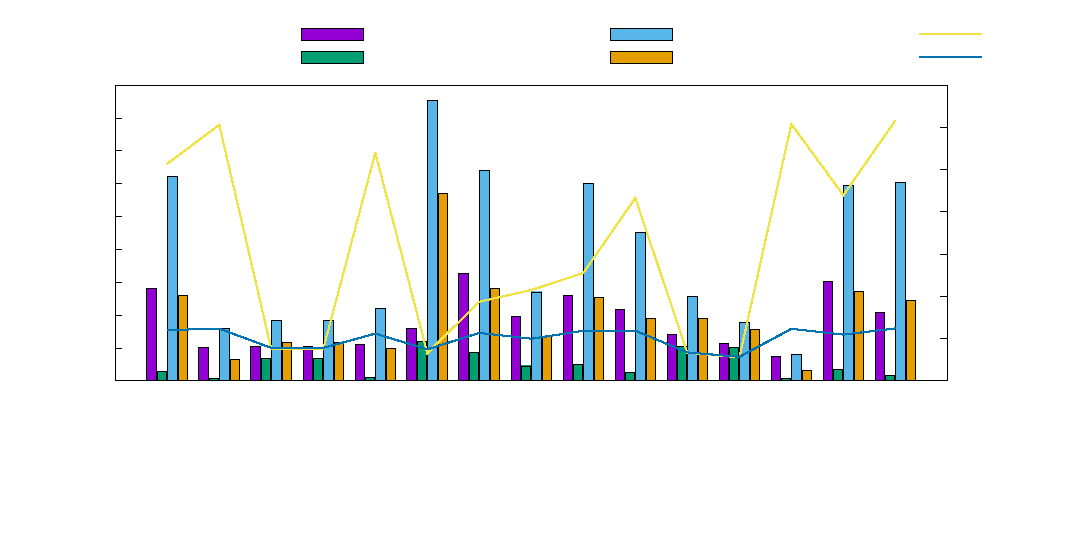
\includegraphics[width={504.00bp},height={252.00bp}]{all-hist-CommunicationMiB}}%
    \gplfronttext
  \end{picture}%
\endgroup

\caption{Communication Size of Benchmarks}
\label{fig:graph_comm_size}
\end{figure*}


\begin{figure*}[htbp]
\centering
% GNUPLOT: LaTeX picture with Postscript
\begingroup
  \makeatletter
  \providecommand\color[2][]{%
    \GenericError{(gnuplot) \space\space\space\@spaces}{%
      Package color not loaded in conjunction with
      terminal option `colourtext'%
    }{See the gnuplot documentation for explanation.%
    }{Either use 'blacktext' in gnuplot or load the package
      color.sty in LaTeX.}%
    \renewcommand\color[2][]{}%
  }%
  \providecommand\includegraphics[2][]{%
    \GenericError{(gnuplot) \space\space\space\@spaces}{%
      Package graphicx or graphics not loaded%
    }{See the gnuplot documentation for explanation.%
    }{The gnuplot epslatex terminal needs graphicx.sty or graphics.sty.}%
    \renewcommand\includegraphics[2][]{}%
  }%
  \providecommand\rotatebox[2]{#2}%
  \@ifundefined{ifGPcolor}{%
    \newif\ifGPcolor
    \GPcolortrue
  }{}%
  \@ifundefined{ifGPblacktext}{%
    \newif\ifGPblacktext
    \GPblacktextfalse
  }{}%
  % define a \g@addto@macro without @ in the name:
  \let\gplgaddtomacro\g@addto@macro
  % define empty templates for all commands taking text:
  \gdef\gplbacktext{}%
  \gdef\gplfronttext{}%
  \makeatother
  \ifGPblacktext
    % no textcolor at all
    \def\colorrgb#1{}%
    \def\colorgray#1{}%
  \else
    % gray or color?
    \ifGPcolor
      \def\colorrgb#1{\color[rgb]{#1}}%
      \def\colorgray#1{\color[gray]{#1}}%
      \expandafter\def\csname LTw\endcsname{\color{white}}%
      \expandafter\def\csname LTb\endcsname{\color{black}}%
      \expandafter\def\csname LTa\endcsname{\color{black}}%
      \expandafter\def\csname LT0\endcsname{\color[rgb]{1,0,0}}%
      \expandafter\def\csname LT1\endcsname{\color[rgb]{0,1,0}}%
      \expandafter\def\csname LT2\endcsname{\color[rgb]{0,0,1}}%
      \expandafter\def\csname LT3\endcsname{\color[rgb]{1,0,1}}%
      \expandafter\def\csname LT4\endcsname{\color[rgb]{0,1,1}}%
      \expandafter\def\csname LT5\endcsname{\color[rgb]{1,1,0}}%
      \expandafter\def\csname LT6\endcsname{\color[rgb]{0,0,0}}%
      \expandafter\def\csname LT7\endcsname{\color[rgb]{1,0.3,0}}%
      \expandafter\def\csname LT8\endcsname{\color[rgb]{0.5,0.5,0.5}}%
    \else
      % gray
      \def\colorrgb#1{\color{black}}%
      \def\colorgray#1{\color[gray]{#1}}%
      \expandafter\def\csname LTw\endcsname{\color{white}}%
      \expandafter\def\csname LTb\endcsname{\color{black}}%
      \expandafter\def\csname LTa\endcsname{\color{black}}%
      \expandafter\def\csname LT0\endcsname{\color{black}}%
      \expandafter\def\csname LT1\endcsname{\color{black}}%
      \expandafter\def\csname LT2\endcsname{\color{black}}%
      \expandafter\def\csname LT3\endcsname{\color{black}}%
      \expandafter\def\csname LT4\endcsname{\color{black}}%
      \expandafter\def\csname LT5\endcsname{\color{black}}%
      \expandafter\def\csname LT6\endcsname{\color{black}}%
      \expandafter\def\csname LT7\endcsname{\color{black}}%
      \expandafter\def\csname LT8\endcsname{\color{black}}%
    \fi
  \fi
    \setlength{\unitlength}{0.0500bp}%
    \ifx\gptboxheight\undefined%
      \newlength{\gptboxheight}%
      \newlength{\gptboxwidth}%
      \newsavebox{\gptboxtext}%
    \fi%
    \setlength{\fboxrule}{0.5pt}%
    \setlength{\fboxsep}{1pt}%
    \definecolor{tbcol}{rgb}{1,1,1}%
\begin{picture}(10080.00,5040.00)%
    \gplgaddtomacro\gplbacktext{%
      \csname LTb\endcsname%%
      \put(814,1100){\makebox(0,0)[r]{\strut{}$0$}}%
      \put(814,1510){\makebox(0,0)[r]{\strut{}$20$}}%
      \put(814,1920){\makebox(0,0)[r]{\strut{}$40$}}%
      \put(814,2330){\makebox(0,0)[r]{\strut{}$60$}}%
      \put(814,2740){\makebox(0,0)[r]{\strut{}$80$}}%
      \put(814,3149){\makebox(0,0)[r]{\strut{}$100$}}%
      \put(814,3559){\makebox(0,0)[r]{\strut{}$120$}}%
      \put(814,3969){\makebox(0,0)[r]{\strut{}$140$}}%
      \put(814,4379){\makebox(0,0)[r]{\strut{}$160$}}%
      \put(1416,968){\rotatebox{-45}{\makebox(0,0)[l]{\strut{}Biometric Distance}}}%
      \put(1886,968){\rotatebox{-45}{\makebox(0,0)[l]{\strut{}Biometric Distance (Fast)}}}%
      \put(2356,968){\rotatebox{-45}{\makebox(0,0)[l]{\strut{}Convex Hull}}}%
      \put(2826,968){\rotatebox{-45}{\makebox(0,0)[l]{\strut{}Count 102}}}%
      \put(3296,968){\rotatebox{-45}{\makebox(0,0)[l]{\strut{}Count 10s}}}%
      \put(3766,968){\rotatebox{-45}{\makebox(0,0)[l]{\strut{}Cryptonets (Max Pooling)}}}%
      \put(4236,968){\rotatebox{-45}{\makebox(0,0)[l]{\strut{}DB Cross Join (Trivial)}}}%
      \put(4706,968){\rotatebox{-45}{\makebox(0,0)[l]{\strut{}Database Variance}}}%
      \put(5175,968){\rotatebox{-45}{\makebox(0,0)[l]{\strut{}Histogram}}}%
      \put(5645,968){\rotatebox{-45}{\makebox(0,0)[l]{\strut{}Inner Product}}}%
      \put(6115,968){\rotatebox{-45}{\makebox(0,0)[l]{\strut{}k-means}}}%
      \put(6585,968){\rotatebox{-45}{\makebox(0,0)[l]{\strut{}Longest 102}}}%
      \put(7055,968){\rotatebox{-45}{\makebox(0,0)[l]{\strut{}Max. Dist. b/w Symbols}}}%
      \put(7525,968){\rotatebox{-45}{\makebox(0,0)[l]{\strut{}Minimal Points}}}%
      \put(7995,968){\rotatebox{-45}{\makebox(0,0)[l]{\strut{}MNIST ReLU}}}%
      \put(8465,968){\rotatebox{-45}{\makebox(0,0)[l]{\strut{}Private Set Intersection}}}%
      \put(9067,1100){\makebox(0,0)[l]{\strut{}$0$}}%
      \put(9067,1568){\makebox(0,0)[l]{\strut{}$10$}}%
      \put(9067,2037){\makebox(0,0)[l]{\strut{}$20$}}%
      \put(9067,2505){\makebox(0,0)[l]{\strut{}$30$}}%
      \put(9067,2974){\makebox(0,0)[l]{\strut{}$40$}}%
      \put(9067,3442){\makebox(0,0)[l]{\strut{}$50$}}%
      \put(9067,3911){\makebox(0,0)[l]{\strut{}$60$}}%
      \put(9067,4379){\makebox(0,0)[l]{\strut{}$70$}}%
    }%
    \gplgaddtomacro\gplfronttext{%
      \csname LTb\endcsname%%
      \put(209,2739){\rotatebox{-270}{\makebox(0,0){\strut{}Circuit Generation Time (sec)}}}%
      \put(9573,2739){\rotatebox{-270}{\makebox(0,0){\strut{}Improvement (number of times)}}}%
      \csname LTb\endcsname%%
      \put(2602,4867){\makebox(0,0)[r]{\strut{}GMW}}%
      \csname LTb\endcsname%%
      \put(2602,4647){\makebox(0,0)[r]{\strut{}GMW (Vectorized)}}%
      \csname LTb\endcsname%%
      \put(5569,4867){\makebox(0,0)[r]{\strut{}BMR}}%
      \csname LTb\endcsname%%
      \put(5569,4647){\makebox(0,0)[r]{\strut{}BMR (Vectorized)}}%
      \csname LTb\endcsname%%
      \put(8536,4867){\makebox(0,0)[r]{\strut{}GMW Improvement}}%
      \csname LTb\endcsname%%
      \put(8536,4647){\makebox(0,0)[r]{\strut{}BMR Improvement}}%
    }%
    \gplbacktext
    \put(0,0){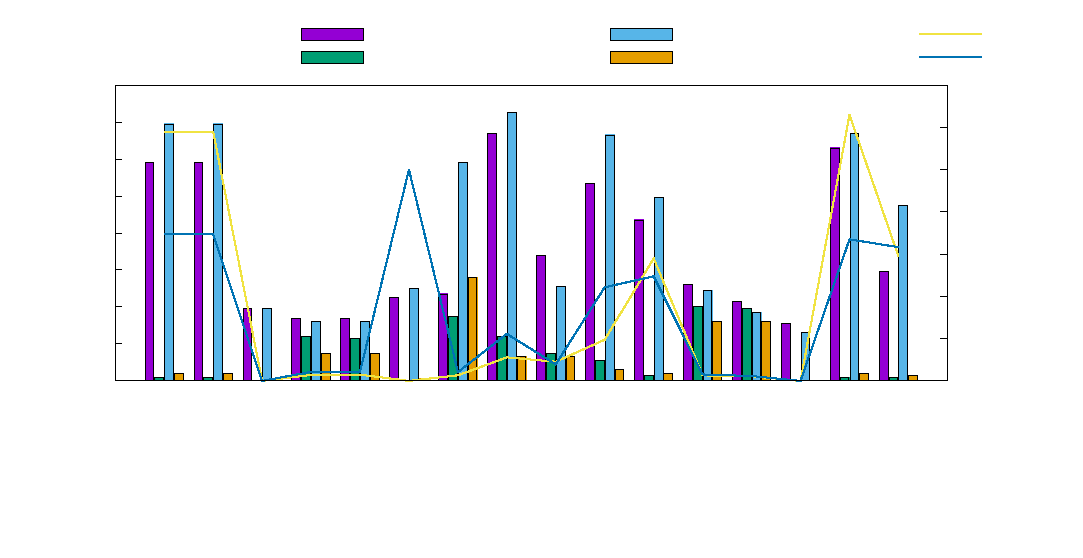
\includegraphics[width={504.00bp},height={252.00bp}]{all-hist-CircuitGenerationTimesec}}%
    \gplfronttext
  \end{picture}%
\endgroup

\caption{Circuit Generation Time of Benchmarks}
\label{fig:graph_circ_gen_time}
\end{figure*}

\begin{figure*}[htbp]
\centering
% GNUPLOT: LaTeX picture with Postscript
\begingroup
  \makeatletter
  \providecommand\color[2][]{%
    \GenericError{(gnuplot) \space\space\space\@spaces}{%
      Package color not loaded in conjunction with
      terminal option `colourtext'%
    }{See the gnuplot documentation for explanation.%
    }{Either use 'blacktext' in gnuplot or load the package
      color.sty in LaTeX.}%
    \renewcommand\color[2][]{}%
  }%
  \providecommand\includegraphics[2][]{%
    \GenericError{(gnuplot) \space\space\space\@spaces}{%
      Package graphicx or graphics not loaded%
    }{See the gnuplot documentation for explanation.%
    }{The gnuplot epslatex terminal needs graphicx.sty or graphics.sty.}%
    \renewcommand\includegraphics[2][]{}%
  }%
  \providecommand\rotatebox[2]{#2}%
  \@ifundefined{ifGPcolor}{%
    \newif\ifGPcolor
    \GPcolortrue
  }{}%
  \@ifundefined{ifGPblacktext}{%
    \newif\ifGPblacktext
    \GPblacktextfalse
  }{}%
  % define a \g@addto@macro without @ in the name:
  \let\gplgaddtomacro\g@addto@macro
  % define empty templates for all commands taking text:
  \gdef\gplbacktext{}%
  \gdef\gplfronttext{}%
  \makeatother
  \ifGPblacktext
    % no textcolor at all
    \def\colorrgb#1{}%
    \def\colorgray#1{}%
  \else
    % gray or color?
    \ifGPcolor
      \def\colorrgb#1{\color[rgb]{#1}}%
      \def\colorgray#1{\color[gray]{#1}}%
      \expandafter\def\csname LTw\endcsname{\color{white}}%
      \expandafter\def\csname LTb\endcsname{\color{black}}%
      \expandafter\def\csname LTa\endcsname{\color{black}}%
      \expandafter\def\csname LT0\endcsname{\color[rgb]{1,0,0}}%
      \expandafter\def\csname LT1\endcsname{\color[rgb]{0,1,0}}%
      \expandafter\def\csname LT2\endcsname{\color[rgb]{0,0,1}}%
      \expandafter\def\csname LT3\endcsname{\color[rgb]{1,0,1}}%
      \expandafter\def\csname LT4\endcsname{\color[rgb]{0,1,1}}%
      \expandafter\def\csname LT5\endcsname{\color[rgb]{1,1,0}}%
      \expandafter\def\csname LT6\endcsname{\color[rgb]{0,0,0}}%
      \expandafter\def\csname LT7\endcsname{\color[rgb]{1,0.3,0}}%
      \expandafter\def\csname LT8\endcsname{\color[rgb]{0.5,0.5,0.5}}%
    \else
      % gray
      \def\colorrgb#1{\color{black}}%
      \def\colorgray#1{\color[gray]{#1}}%
      \expandafter\def\csname LTw\endcsname{\color{white}}%
      \expandafter\def\csname LTb\endcsname{\color{black}}%
      \expandafter\def\csname LTa\endcsname{\color{black}}%
      \expandafter\def\csname LT0\endcsname{\color{black}}%
      \expandafter\def\csname LT1\endcsname{\color{black}}%
      \expandafter\def\csname LT2\endcsname{\color{black}}%
      \expandafter\def\csname LT3\endcsname{\color{black}}%
      \expandafter\def\csname LT4\endcsname{\color{black}}%
      \expandafter\def\csname LT5\endcsname{\color{black}}%
      \expandafter\def\csname LT6\endcsname{\color{black}}%
      \expandafter\def\csname LT7\endcsname{\color{black}}%
      \expandafter\def\csname LT8\endcsname{\color{black}}%
    \fi
  \fi
    \setlength{\unitlength}{0.0500bp}%
    \ifx\gptboxheight\undefined%
      \newlength{\gptboxheight}%
      \newlength{\gptboxwidth}%
      \newsavebox{\gptboxtext}%
    \fi%
    \setlength{\fboxrule}{0.5pt}%
    \setlength{\fboxsep}{1pt}%
    \definecolor{tbcol}{rgb}{1,1,1}%
\begin{picture}(10080.00,5040.00)%
    \gplgaddtomacro\gplbacktext{%
      \csname LTb\endcsname%%
      \put(1342,1100){\makebox(0,0)[r]{\strut{}$0$}}%
      \put(1342,1756){\makebox(0,0)[r]{\strut{}$500000$}}%
      \put(1342,2412){\makebox(0,0)[r]{\strut{}$1\times10^{6}$}}%
      \put(1342,3067){\makebox(0,0)[r]{\strut{}$1.5\times10^{6}$}}%
      \put(1342,3723){\makebox(0,0)[r]{\strut{}$2\times10^{6}$}}%
      \put(1342,4379){\makebox(0,0)[r]{\strut{}$2.5\times10^{6}$}}%
      \put(1905,968){\rotatebox{-45}{\makebox(0,0)[l]{\strut{}Biometric Distance}}}%
      \put(2336,968){\rotatebox{-45}{\makebox(0,0)[l]{\strut{}Biometric Distance (Fast)}}}%
      \put(2767,968){\rotatebox{-45}{\makebox(0,0)[l]{\strut{}Convex Hull}}}%
      \put(3198,968){\rotatebox{-45}{\makebox(0,0)[l]{\strut{}Count 102}}}%
      \put(3630,968){\rotatebox{-45}{\makebox(0,0)[l]{\strut{}Count 10s}}}%
      \put(4061,968){\rotatebox{-45}{\makebox(0,0)[l]{\strut{}Cryptonets (Max Pooling)}}}%
      \put(4492,968){\rotatebox{-45}{\makebox(0,0)[l]{\strut{}DB Cross Join (Trivial)}}}%
      \put(4923,968){\rotatebox{-45}{\makebox(0,0)[l]{\strut{}Database Variance}}}%
      \put(5354,968){\rotatebox{-45}{\makebox(0,0)[l]{\strut{}Histogram}}}%
      \put(5785,968){\rotatebox{-45}{\makebox(0,0)[l]{\strut{}Inner Product}}}%
      \put(6216,968){\rotatebox{-45}{\makebox(0,0)[l]{\strut{}k-means}}}%
      \put(6647,968){\rotatebox{-45}{\makebox(0,0)[l]{\strut{}Longest 102}}}%
      \put(7079,968){\rotatebox{-45}{\makebox(0,0)[l]{\strut{}Max. Dist. b/w Symbols}}}%
      \put(7510,968){\rotatebox{-45}{\makebox(0,0)[l]{\strut{}Minimal Points}}}%
      \put(7941,968){\rotatebox{-45}{\makebox(0,0)[l]{\strut{}MNIST ReLU}}}%
      \put(8372,968){\rotatebox{-45}{\makebox(0,0)[l]{\strut{}Private Set Intersection}}}%
      \put(8935,1100){\makebox(0,0)[l]{\strut{}$0$}}%
      \put(8935,1428){\makebox(0,0)[l]{\strut{}$50$}}%
      \put(8935,1756){\makebox(0,0)[l]{\strut{}$100$}}%
      \put(8935,2084){\makebox(0,0)[l]{\strut{}$150$}}%
      \put(8935,2412){\makebox(0,0)[l]{\strut{}$200$}}%
      \put(8935,2740){\makebox(0,0)[l]{\strut{}$250$}}%
      \put(8935,3067){\makebox(0,0)[l]{\strut{}$300$}}%
      \put(8935,3395){\makebox(0,0)[l]{\strut{}$350$}}%
      \put(8935,3723){\makebox(0,0)[l]{\strut{}$400$}}%
      \put(8935,4051){\makebox(0,0)[l]{\strut{}$450$}}%
      \put(8935,4379){\makebox(0,0)[l]{\strut{}$500$}}%
    }%
    \gplgaddtomacro\gplfronttext{%
      \csname LTb\endcsname%%
      \put(209,2739){\rotatebox{-270}{\makebox(0,0){\strut{}Total Gates}}}%
      \put(9573,2739){\rotatebox{-270}{\makebox(0,0){\strut{}Improvement (number of times)}}}%
      \csname LTb\endcsname%%
      \put(2800,4867){\makebox(0,0)[r]{\strut{}GMW}}%
      \csname LTb\endcsname%%
      \put(2800,4647){\makebox(0,0)[r]{\strut{}GMW (Vectorized)}}%
      \csname LTb\endcsname%%
      \put(5767,4867){\makebox(0,0)[r]{\strut{}BMR}}%
      \csname LTb\endcsname%%
      \put(5767,4647){\makebox(0,0)[r]{\strut{}BMR (Vectorized)}}%
      \csname LTb\endcsname%%
      \put(8734,4867){\makebox(0,0)[r]{\strut{}GMW Improvement}}%
      \csname LTb\endcsname%%
      \put(8734,4647){\makebox(0,0)[r]{\strut{}BMR Improvement}}%
    }%
    \gplbacktext
    \put(0,0){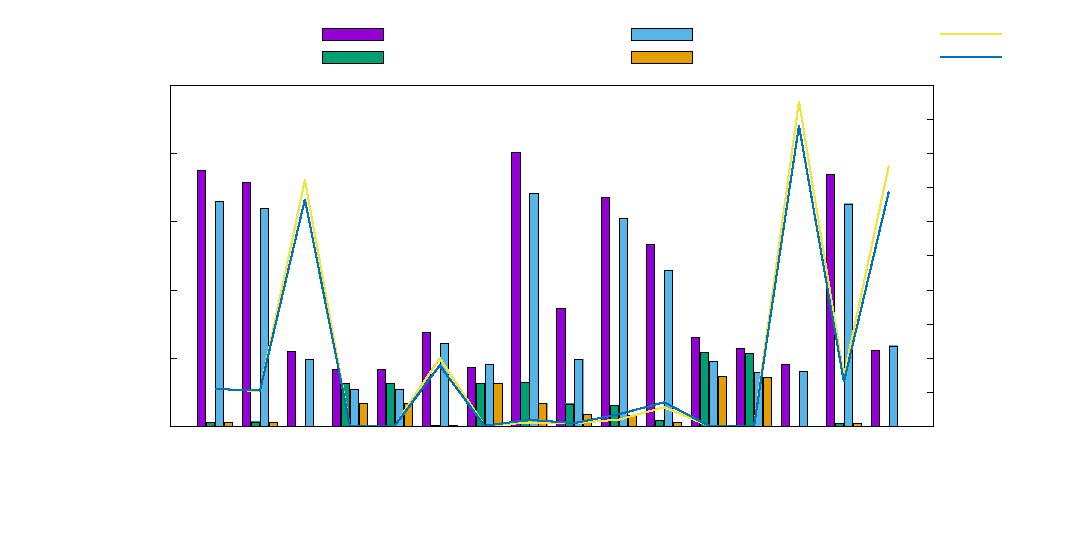
\includegraphics[width={504.00bp},height={252.00bp}]{all-hist-TotalGates}}%
    \gplfronttext
  \end{picture}%
\endgroup

\caption{Number of Gates of Benchmarks}
\label{fig:graph_total_gates}
\end{figure*}

\begin{figure*}[htbp]
\centering
% GNUPLOT: LaTeX picture with Postscript
\begingroup
  \makeatletter
  \providecommand\color[2][]{%
    \GenericError{(gnuplot) \space\space\space\@spaces}{%
      Package color not loaded in conjunction with
      terminal option `colourtext'%
    }{See the gnuplot documentation for explanation.%
    }{Either use 'blacktext' in gnuplot or load the package
      color.sty in LaTeX.}%
    \renewcommand\color[2][]{}%
  }%
  \providecommand\includegraphics[2][]{%
    \GenericError{(gnuplot) \space\space\space\@spaces}{%
      Package graphicx or graphics not loaded%
    }{See the gnuplot documentation for explanation.%
    }{The gnuplot epslatex terminal needs graphicx.sty or graphics.sty.}%
    \renewcommand\includegraphics[2][]{}%
  }%
  \providecommand\rotatebox[2]{#2}%
  \@ifundefined{ifGPcolor}{%
    \newif\ifGPcolor
    \GPcolortrue
  }{}%
  \@ifundefined{ifGPblacktext}{%
    \newif\ifGPblacktext
    \GPblacktextfalse
  }{}%
  % define a \g@addto@macro without @ in the name:
  \let\gplgaddtomacro\g@addto@macro
  % define empty templates for all commands taking text:
  \gdef\gplbacktext{}%
  \gdef\gplfronttext{}%
  \makeatother
  \ifGPblacktext
    % no textcolor at all
    \def\colorrgb#1{}%
    \def\colorgray#1{}%
  \else
    % gray or color?
    \ifGPcolor
      \def\colorrgb#1{\color[rgb]{#1}}%
      \def\colorgray#1{\color[gray]{#1}}%
      \expandafter\def\csname LTw\endcsname{\color{white}}%
      \expandafter\def\csname LTb\endcsname{\color{black}}%
      \expandafter\def\csname LTa\endcsname{\color{black}}%
      \expandafter\def\csname LT0\endcsname{\color[rgb]{1,0,0}}%
      \expandafter\def\csname LT1\endcsname{\color[rgb]{0,1,0}}%
      \expandafter\def\csname LT2\endcsname{\color[rgb]{0,0,1}}%
      \expandafter\def\csname LT3\endcsname{\color[rgb]{1,0,1}}%
      \expandafter\def\csname LT4\endcsname{\color[rgb]{0,1,1}}%
      \expandafter\def\csname LT5\endcsname{\color[rgb]{1,1,0}}%
      \expandafter\def\csname LT6\endcsname{\color[rgb]{0,0,0}}%
      \expandafter\def\csname LT7\endcsname{\color[rgb]{1,0.3,0}}%
      \expandafter\def\csname LT8\endcsname{\color[rgb]{0.5,0.5,0.5}}%
    \else
      % gray
      \def\colorrgb#1{\color{black}}%
      \def\colorgray#1{\color[gray]{#1}}%
      \expandafter\def\csname LTw\endcsname{\color{white}}%
      \expandafter\def\csname LTb\endcsname{\color{black}}%
      \expandafter\def\csname LTa\endcsname{\color{black}}%
      \expandafter\def\csname LT0\endcsname{\color{black}}%
      \expandafter\def\csname LT1\endcsname{\color{black}}%
      \expandafter\def\csname LT2\endcsname{\color{black}}%
      \expandafter\def\csname LT3\endcsname{\color{black}}%
      \expandafter\def\csname LT4\endcsname{\color{black}}%
      \expandafter\def\csname LT5\endcsname{\color{black}}%
      \expandafter\def\csname LT6\endcsname{\color{black}}%
      \expandafter\def\csname LT7\endcsname{\color{black}}%
      \expandafter\def\csname LT8\endcsname{\color{black}}%
    \fi
  \fi
    \setlength{\unitlength}{0.0500bp}%
    \ifx\gptboxheight\undefined%
      \newlength{\gptboxheight}%
      \newlength{\gptboxwidth}%
      \newsavebox{\gptboxtext}%
    \fi%
    \setlength{\fboxrule}{0.5pt}%
    \setlength{\fboxsep}{1pt}%
    \definecolor{tbcol}{rgb}{1,1,1}%
\begin{picture}(10080.00,5040.00)%
    \gplgaddtomacro\gplbacktext{%
      \csname LTb\endcsname%%
      \put(814,1540){\makebox(0,0)[r]{\strut{}$0$}}%
      \put(814,1855){\makebox(0,0)[r]{\strut{}$20$}}%
      \put(814,2171){\makebox(0,0)[r]{\strut{}$40$}}%
      \put(814,2486){\makebox(0,0)[r]{\strut{}$60$}}%
      \put(814,2802){\makebox(0,0)[r]{\strut{}$80$}}%
      \put(814,3117){\makebox(0,0)[r]{\strut{}$100$}}%
      \put(814,3433){\makebox(0,0)[r]{\strut{}$120$}}%
      \put(814,3748){\makebox(0,0)[r]{\strut{}$140$}}%
      \put(814,4064){\makebox(0,0)[r]{\strut{}$160$}}%
      \put(814,4379){\makebox(0,0)[r]{\strut{}$180$}}%
      \put(1408,1408){\rotatebox{-45}{\makebox(0,0)[l]{\strut{}Biometric Matching}}}%
      \put(1870,1408){\rotatebox{-45}{\makebox(0,0)[l]{\strut{}Biometric Matching (Fast)}}}%
      \put(2333,1408){\rotatebox{-45}{\makebox(0,0)[l]{\strut{}Convex Hull}}}%
      \put(2795,1408){\rotatebox{-45}{\makebox(0,0)[l]{\strut{}Count 102}}}%
      \put(3257,1408){\rotatebox{-45}{\makebox(0,0)[l]{\strut{}Count 10s}}}%
      \put(3719,1408){\rotatebox{-45}{\makebox(0,0)[l]{\strut{}Cryptonets (Max Pooling)}}}%
      \put(4181,1408){\rotatebox{-45}{\makebox(0,0)[l]{\strut{}Database Join}}}%
      \put(4643,1408){\rotatebox{-45}{\makebox(0,0)[l]{\strut{}Database Variance}}}%
      \put(5106,1408){\rotatebox{-45}{\makebox(0,0)[l]{\strut{}Histogram}}}%
      \put(5568,1408){\rotatebox{-45}{\makebox(0,0)[l]{\strut{}Inner Product}}}%
      \put(6030,1408){\rotatebox{-45}{\makebox(0,0)[l]{\strut{}k-means}}}%
      \put(6492,1408){\rotatebox{-45}{\makebox(0,0)[l]{\strut{}Longest 102}}}%
      \put(6954,1408){\rotatebox{-45}{\makebox(0,0)[l]{\strut{}Max. Dist. b/w Symbols}}}%
      \put(7416,1408){\rotatebox{-45}{\makebox(0,0)[l]{\strut{}Minimal Points}}}%
      \put(7879,1408){\rotatebox{-45}{\makebox(0,0)[l]{\strut{}MNIST ReLU}}}%
      \put(8341,1408){\rotatebox{-45}{\makebox(0,0)[l]{\strut{}Private Set Intersection}}}%
      \put(8935,1540){\makebox(0,0)[l]{\strut{}$0$}}%
      \put(8935,1895){\makebox(0,0)[l]{\strut{}$20$}}%
      \put(8935,2250){\makebox(0,0)[l]{\strut{}$40$}}%
      \put(8935,2605){\makebox(0,0)[l]{\strut{}$60$}}%
      \put(8935,2960){\makebox(0,0)[l]{\strut{}$80$}}%
      \put(8935,3314){\makebox(0,0)[l]{\strut{}$100$}}%
      \put(8935,3669){\makebox(0,0)[l]{\strut{}$120$}}%
      \put(8935,4024){\makebox(0,0)[l]{\strut{}$140$}}%
      \put(8935,4379){\makebox(0,0)[l]{\strut{}$160$}}%
    }%
    \gplgaddtomacro\gplfronttext{%
      \csname LTb\endcsname%%
      \put(209,2959){\rotatebox{-270}{\makebox(0,0){\strut{}Online Time (sec)}}}%
      \put(9573,2959){\rotatebox{-270}{\makebox(0,0){\strut{}Improvement (number of times)}}}%
      \csname LTb\endcsname%%
      \put(2536,4867){\makebox(0,0)[r]{\strut{}GMW}}%
      \csname LTb\endcsname%%
      \put(2536,4647){\makebox(0,0)[r]{\strut{}GMW (Vectorized)}}%
      \csname LTb\endcsname%%
      \put(5503,4867){\makebox(0,0)[r]{\strut{}BMR}}%
      \csname LTb\endcsname%%
      \put(5503,4647){\makebox(0,0)[r]{\strut{}BMR (Vectorized)}}%
      \csname LTb\endcsname%%
      \put(8470,4867){\makebox(0,0)[r]{\strut{}GMW Improvement}}%
      \csname LTb\endcsname%%
      \put(8470,4647){\makebox(0,0)[r]{\strut{}BMR Improvement}}%
    }%
    \gplbacktext
    \put(0,0){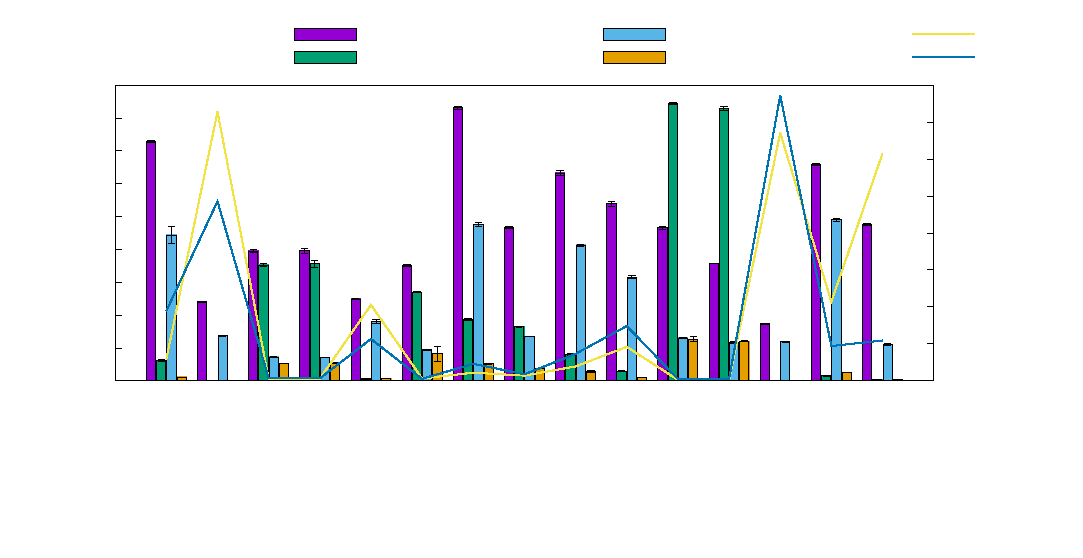
\includegraphics[width={504.00bp},height={252.00bp}]{all-hist-OnlineTimesec}}%
    \gplfronttext
  \end{picture}%
\endgroup

\caption{Online Time of Benchmarks}
\label{fig:graph_online_time}
\end{figure*}

\begin{figure*}[htbp]
\centering
% GNUPLOT: LaTeX picture with Postscript
\begingroup
  \makeatletter
  \providecommand\color[2][]{%
    \GenericError{(gnuplot) \space\space\space\@spaces}{%
      Package color not loaded in conjunction with
      terminal option `colourtext'%
    }{See the gnuplot documentation for explanation.%
    }{Either use 'blacktext' in gnuplot or load the package
      color.sty in LaTeX.}%
    \renewcommand\color[2][]{}%
  }%
  \providecommand\includegraphics[2][]{%
    \GenericError{(gnuplot) \space\space\space\@spaces}{%
      Package graphicx or graphics not loaded%
    }{See the gnuplot documentation for explanation.%
    }{The gnuplot epslatex terminal needs graphicx.sty or graphics.sty.}%
    \renewcommand\includegraphics[2][]{}%
  }%
  \providecommand\rotatebox[2]{#2}%
  \@ifundefined{ifGPcolor}{%
    \newif\ifGPcolor
    \GPcolortrue
  }{}%
  \@ifundefined{ifGPblacktext}{%
    \newif\ifGPblacktext
    \GPblacktextfalse
  }{}%
  % define a \g@addto@macro without @ in the name:
  \let\gplgaddtomacro\g@addto@macro
  % define empty templates for all commands taking text:
  \gdef\gplbacktext{}%
  \gdef\gplfronttext{}%
  \makeatother
  \ifGPblacktext
    % no textcolor at all
    \def\colorrgb#1{}%
    \def\colorgray#1{}%
  \else
    % gray or color?
    \ifGPcolor
      \def\colorrgb#1{\color[rgb]{#1}}%
      \def\colorgray#1{\color[gray]{#1}}%
      \expandafter\def\csname LTw\endcsname{\color{white}}%
      \expandafter\def\csname LTb\endcsname{\color{black}}%
      \expandafter\def\csname LTa\endcsname{\color{black}}%
      \expandafter\def\csname LT0\endcsname{\color[rgb]{1,0,0}}%
      \expandafter\def\csname LT1\endcsname{\color[rgb]{0,1,0}}%
      \expandafter\def\csname LT2\endcsname{\color[rgb]{0,0,1}}%
      \expandafter\def\csname LT3\endcsname{\color[rgb]{1,0,1}}%
      \expandafter\def\csname LT4\endcsname{\color[rgb]{0,1,1}}%
      \expandafter\def\csname LT5\endcsname{\color[rgb]{1,1,0}}%
      \expandafter\def\csname LT6\endcsname{\color[rgb]{0,0,0}}%
      \expandafter\def\csname LT7\endcsname{\color[rgb]{1,0.3,0}}%
      \expandafter\def\csname LT8\endcsname{\color[rgb]{0.5,0.5,0.5}}%
    \else
      % gray
      \def\colorrgb#1{\color{black}}%
      \def\colorgray#1{\color[gray]{#1}}%
      \expandafter\def\csname LTw\endcsname{\color{white}}%
      \expandafter\def\csname LTb\endcsname{\color{black}}%
      \expandafter\def\csname LTa\endcsname{\color{black}}%
      \expandafter\def\csname LT0\endcsname{\color{black}}%
      \expandafter\def\csname LT1\endcsname{\color{black}}%
      \expandafter\def\csname LT2\endcsname{\color{black}}%
      \expandafter\def\csname LT3\endcsname{\color{black}}%
      \expandafter\def\csname LT4\endcsname{\color{black}}%
      \expandafter\def\csname LT5\endcsname{\color{black}}%
      \expandafter\def\csname LT6\endcsname{\color{black}}%
      \expandafter\def\csname LT7\endcsname{\color{black}}%
      \expandafter\def\csname LT8\endcsname{\color{black}}%
    \fi
  \fi
    \setlength{\unitlength}{0.0500bp}%
    \ifx\gptboxheight\undefined%
      \newlength{\gptboxheight}%
      \newlength{\gptboxwidth}%
      \newsavebox{\gptboxtext}%
    \fi%
    \setlength{\fboxrule}{0.5pt}%
    \setlength{\fboxsep}{1pt}%
    \definecolor{tbcol}{rgb}{1,1,1}%
\begin{picture}(10080.00,5040.00)%
    \gplgaddtomacro\gplbacktext{%
      \csname LTb\endcsname%%
      \put(814,1540){\makebox(0,0)[r]{\strut{}$0$}}%
      \put(814,2013){\makebox(0,0)[r]{\strut{}$50$}}%
      \put(814,2486){\makebox(0,0)[r]{\strut{}$100$}}%
      \put(814,2960){\makebox(0,0)[r]{\strut{}$150$}}%
      \put(814,3433){\makebox(0,0)[r]{\strut{}$200$}}%
      \put(814,3906){\makebox(0,0)[r]{\strut{}$250$}}%
      \put(814,4379){\makebox(0,0)[r]{\strut{}$300$}}%
      \put(1445,1408){\rotatebox{-45}{\makebox(0,0)[l]{\strut{}Biometric Matching}}}%
      \put(1945,1408){\rotatebox{-45}{\makebox(0,0)[l]{\strut{}Convex Hull}}}%
      \put(2444,1408){\rotatebox{-45}{\makebox(0,0)[l]{\strut{}Count 102}}}%
      \put(2943,1408){\rotatebox{-45}{\makebox(0,0)[l]{\strut{}Count 10s}}}%
      \put(3443,1408){\rotatebox{-45}{\makebox(0,0)[l]{\strut{}Cryptonets (Max Pooling)}}}%
      \put(3942,1408){\rotatebox{-45}{\makebox(0,0)[l]{\strut{}Database Join}}}%
      \put(4441,1408){\rotatebox{-45}{\makebox(0,0)[l]{\strut{}Database Variance}}}%
      \put(4941,1408){\rotatebox{-45}{\makebox(0,0)[l]{\strut{}Histogram}}}%
      \put(5440,1408){\rotatebox{-45}{\makebox(0,0)[l]{\strut{}Inner Product}}}%
      \put(5939,1408){\rotatebox{-45}{\makebox(0,0)[l]{\strut{}k-means}}}%
      \put(6438,1408){\rotatebox{-45}{\makebox(0,0)[l]{\strut{}Longest 102}}}%
      \put(6938,1408){\rotatebox{-45}{\makebox(0,0)[l]{\strut{}Max. Dist. b/w Symbols}}}%
      \put(7437,1408){\rotatebox{-45}{\makebox(0,0)[l]{\strut{}Minimal Points}}}%
      \put(7936,1408){\rotatebox{-45}{\makebox(0,0)[l]{\strut{}MNIST ReLU}}}%
      \put(8436,1408){\rotatebox{-45}{\makebox(0,0)[l]{\strut{}Private Set Intersection}}}%
      \put(9067,1540){\makebox(0,0)[l]{\strut{}$0$}}%
      \put(9067,1946){\makebox(0,0)[l]{\strut{}$5$}}%
      \put(9067,2351){\makebox(0,0)[l]{\strut{}$10$}}%
      \put(9067,2757){\makebox(0,0)[l]{\strut{}$15$}}%
      \put(9067,3162){\makebox(0,0)[l]{\strut{}$20$}}%
      \put(9067,3568){\makebox(0,0)[l]{\strut{}$25$}}%
      \put(9067,3973){\makebox(0,0)[l]{\strut{}$30$}}%
      \put(9067,4379){\makebox(0,0)[l]{\strut{}$35$}}%
    }%
    \gplgaddtomacro\gplfronttext{%
      \csname LTb\endcsname%%
      \put(209,2959){\rotatebox{-270}{\makebox(0,0){\strut{}Setup Time (sec)}}}%
      \put(9573,2959){\rotatebox{-270}{\makebox(0,0){\strut{}Improvement (number of times)}}}%
      \csname LTb\endcsname%%
      \put(2602,4867){\makebox(0,0)[r]{\strut{}GMW}}%
      \csname LTb\endcsname%%
      \put(2602,4647){\makebox(0,0)[r]{\strut{}GMW (Vectorized)}}%
      \csname LTb\endcsname%%
      \put(5569,4867){\makebox(0,0)[r]{\strut{}BMR}}%
      \csname LTb\endcsname%%
      \put(5569,4647){\makebox(0,0)[r]{\strut{}BMR (Vectorized)}}%
      \csname LTb\endcsname%%
      \put(8536,4867){\makebox(0,0)[r]{\strut{}GMW Improvement}}%
      \csname LTb\endcsname%%
      \put(8536,4647){\makebox(0,0)[r]{\strut{}BMR Improvement}}%
    }%
    \gplbacktext
    \put(0,0){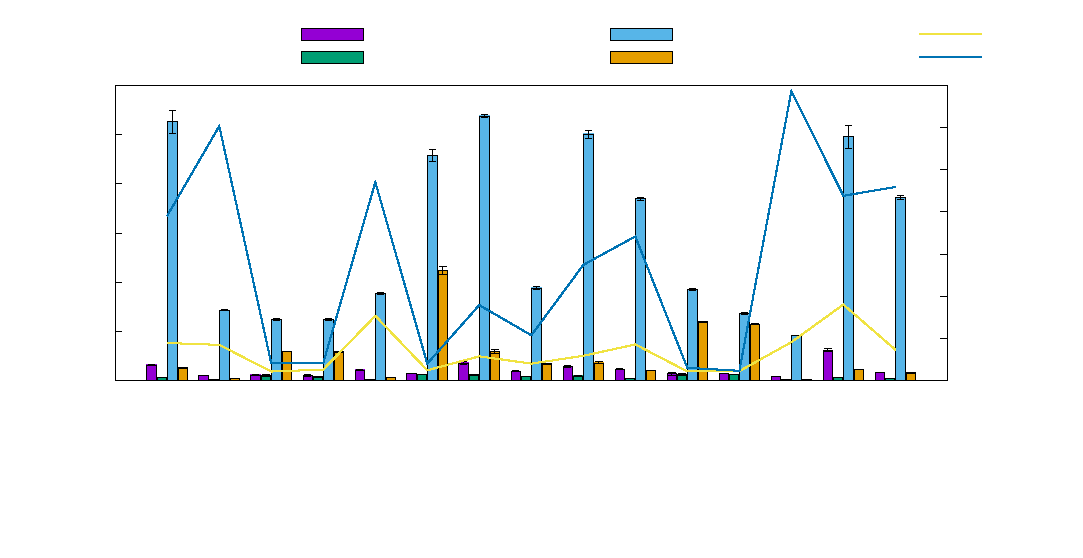
\includegraphics[width={504.00bp},height={252.00bp}]{all-hist-SetupTimesec}}%
    \gplfronttext
  \end{picture}%
\endgroup

\caption{Setup Time of Benchmarks}
\label{fig:graph_setup_time}
\end{figure*}

\subsection{Comparison with MOTION-native Inner Product and Discussion}

%We conclude the . 
Finally, we compared our automatically generated routine for Inner Product with the manually SIMD-ified MOTION-native routine in the distribution. 
We were surprised that we were an order of magnitude slower in Boolean GMW as our circuit ran a significantly larger 
number of communication rounds. Upon investigation, it turned out that the vectorized multiplications were essentially the same, 
however, our addition loop incurred significant cost (ADD is non-local and expensive in Boolean GMW). The MOTION-native loop ran 
{\sf result += mult\_unsimdified[i];} while our loop generated and ran {\sf result[i] = result[i] + mult\_unsimdified[i];}. 
We rewrote the accumulation (manually, for testing purposes) and that led to the comparable speedup!

Therefore, MOTION's compiler performs analysis that informs circuit generation. In the above example, 
MOTION does the standard divide-and-conquer accumulation. The example also illustrates the limitation of higher-level AST analysis --- while 
the analysis was able to detect the associative accumulation when operator {\sf += } was used, it was unable to do so when an equivalent 
code was used. We conjecture that MPC source, as a more straight-forward representation will
not only enable detection of general associative loops, but also allow for program synthesis to increase opportunities for divide-and-conquer
parallelization~\cite{Farzan:2021}; we leave this as future work. 

The most closely related work, HyCC~\cite{CCS:BDKKS18}, is a mixing compiler that focuses on mixed protocols, while we run vectorization within a single protocol. 
The paper only provides data for Boolean and Yao for a version of Biometric matching on $N=1000$; it does provide a lot of data on mixed protocol executions.
Again, we estimate we are about an order of magnitude slower. This is likely due to the same issue as Inner Product --- the computation of min can be optimized. 



%\ana{Ana todo: Discuss why we are slower than HyCC --- because of ad-hoc div-and-conquer optimizations. Have to summarize what Ben and I figured out yesterday.}

%\ana{If we can add that our cost model works great (it does!), that would be great but probably won't have time...}
